% !TeX encoding = UTF-8
% !TeX spellcheck = en_GB
% !TeX program = lualatex
% !TeX TXS-program:bibliography = txs:///bibtex
% !BIB program = bibtex
% !TeX root=manual.tex
% \pdfminorversion=4
\documentclass[oneside, 10pt]{scrbook}


% !TeX encoding = UTF-8 Unicode
% !TeX root = manual.tex
% !TeX spellcheck = en_GB

%Babel zuerst
%===============
%\usepackage[utf8]{inputenc}
\usepackage[ngerman,english]{babel}		%ngerman für Neue Deutsche Rechtschreibung, english für Englisch
\def\ensuretext{\textrm}



\usepackage{graphicx}
%\usepackage{hyperref}



\setcounter{secnumdepth}{1}
\setcounter{tocdepth}{2}

%=============================================
\usepackage{amsmath, amsthm, amssymb, amsfonts, mathtools}
\usepackage[a4paper, top=3cm, bottom=3cm, left=2cm, right=2cm]{geometry}
\usepackage{xcolor}
%\usepackage[verbose]{placeins}	%Verhinder Floating über subsections
\usepackage{graphicx}
\usepackage[autostyle=true]{csquotes}
\usepackage{mathdots} %Rede­fines \ddots and \vdots, and de­fines \id­dots.
\usepackage{upquote} %needed for correct quotes in the listings
\usepackage{listings}

\usepackage[inline]{enumitem} %For enumeration
\newlist{param}{description}{10}
\setlist[param]{style=unboxed, font=\texttt, labelindent=\parindent,leftmargin=*, itemsep=0ex, itemindent=!}
%\usepackage{upquote}
%\usepackage{multicol}

%\usepackage{soul}		%um gesperrt zu schreiben mit Befehl \so{gesperrter Text} 
%\usepackage[inline]{enumitem}
%\usepackage{cnenum}

\usepackage[bookmarks=true, breaklinks=true, colorlinks=false, pdfborder={0 0 0}, pdfa, draft=false]{hyperref} 
\providecommand\phantomsection{} %allows to comment out hyperref package
% Optionen weg wenn was nicht geht, Muss als letztes Package da stehn




%Design Änderungen, Compile Änderungen
%=======================================
%Sorgt dafuer, dass Bilder erst auf einzelner Seite stehn wenn weniger als 20% Text darauf waer
%\renewcommand{\floatpagefraction}{0.8}	
\vfuzz2pt                 % Don't report over-full v-boxes if over-edge is small
\hfuzz2pt                 % Don't report over-full h-boxes if over-edge is small

                          
%Weitere Wichtige Befehle
%==========================
\definecolor{darkyellow}{rgb}{0.65, 0.5, 0.05}
\definecolor{darkgreen}{rgb}{0.05, 0.5, 0.05}
\newcommand{\XX}[1]{%
    {\color{red}\footnotesize%
    \phantomsection\addcontentsline{lof}{section}{\protect\framebox{\textbf{XX}}\protect\color{red} #1}%
    \framebox{\textbf{XX}}\emph{\textbf{#1}}}}%


%%%%%%%%%%%%%%%%%%%
% Specific stuff
%%%%%%%%%%%%%%%%%%%%%%

\newcommand{\fwsym}[1]{\parbox[c]{.9em}{\protect\ensuremath{#1}}}
\newcommand{\ppmm}{\fwsym{\pm}}
\newcommand{\Circ}{{\raisebox{-0.2ex}{\scalebox{1.4}{$\circ$}}}}
\newcommand{\pp}{\fwsym{+}}
\newcommand{\mm}{\fwsym{-}}
\newcommand{\nn}{\fwsym{\Circ}}
\newcommand{\seqj}[0]{{\,\boldsymbol{j}}}
\newcommand{\nablal}[0]{{\nabla_{\!l}\,}}
\newcommand{\nablak}[0]{{\nabla^{k}\,}}
\newcommand{\nablakp}[0]{{\nabla^{k+1}\,}}
\newcommand{\nablamu}[0]{{\tilde{\nabla}^{\mu}\,}}
\newcommand{\assS}[0]{\ensuretext{\textbf{S}}}
%\newcommand{\coast}{\operatorname{co}_\ast}
%\DeclareMathOperator{\hausdorff}{h}

\newcommand{\FWFtext}[1]{{\color{gray}#1}}

\let\subsetneq\undefined %undefine subsetneq, since we only want to use \subsetneqq
\let\subset\undefined %undefine subset, since we only want to use \subseteq

\DeclareMathOperator{\JSR}{JSR}
\DeclareMathOperator{\LSR}{LSR}
\DeclareMathOperator{\RSR}{RSR}
\DeclareMathOperator{\capacity}{cap}

%\swapnumbers %To write the numbers before Theorem/Definition/...

%%%%%% Redefine :=
%\mathchardef\ordinarycolon\mathcode`\:
%\mathcode`\:=\string"8000
%\begingroup \catcode`\:=\active
%  \gdef:{\mathrel{\mathop\ordinarycolon}}
%\endgroup

\numberwithin{equation}{section}

\hyphenation{bal-anc-ing}
\hyphenation{Dau-bechies}
\hyphenation{wave-lets}
\hyphenation{wave-let}

%%%%%%%%%%%%%%%
% Mathematical stuff
%%%%%%%%%%%%%%%
%
%Theorems
%=======================

\newtheorem{theorem}{Theorem}[section]
\newtheorem{lemma}[theorem]{Lemma}
\newtheorem{assumption}[theorem]{Assumption}
\newtheorem{proposition}[theorem]{Proposition}
\newtheorem{corollary}[theorem]{Corollary}
%\newtheorem{claim}[theorem]{Claim}
\newtheorem{conjecture}[theorem]{Conjecture}
\newtheorem{goal}{Goal}[]

\theoremstyle{definition}
%\newtheorem*{claim*}{Claim}
\newtheorem{definition}[theorem]{Definition}
\newtheorem{remark}[theorem]{Remark}
\newtheorem{example}[theorem]{Example}
\newtheorem{algorithm}[theorem]{Algorithm}
\newtheorem{algdef}[theorem]{Algorithm and Definition}

%\newtheorem{exampleX}[theorem]{Example}
%\newcommand{\examplesymbol}{\ensuremath{\triangle}}
%\newenvironment{example}%To add a symbol at the end of the example environment
%{%
%    \pushQED{\qed}%
%    \renewcommand{\qedsymbol}{\examplesymbol}
%    \exampleX%
%}
%{
%    \popQED%
%    \endexampleX%
%}%

%% Various commands
%=======================
\newcommand\numberthis{\addtocounter{equation}{1}\tag{\theequation}}
%\newcommand{\pbrackets}[1]{\left( #1 \right)}
%\newcommand{\Pbrackets}[1]{\left( #1 \vphantom{\left(#1\right)^A} \right)}
\newcommand*\justify{% for texttt % use as \texttt{\justify lorem ip sum)},
%  \fontdimen2\font=0.4em% interword space
%  \fontdimen3\font=0.2em% interword stretch
%  \fontdimen4\font=0.1em% interword shrink
%  \fontdimen7\font=0.1em% extra space
  \hyphenchar\font=`\-% allowing hyphenation
}



%% Symbols of functions
%====================
%\DeclareMathOperator{\FT}{\mathcal{F}}
\DeclareMathOperator{\spn}{span}
\DeclareMathOperator{\supp}{supp}
\newcommand{\lebesgue}[1]{\lambda\left( #1 \right)} \let\lebesgue\lebesgue
\newcommand{\Fourierhat}[1]{#1\!\widehat{\phantom{x}}} \let\Fourierhat\Fourierhat  %Fourier-Transform Sign with hat
\newcommand{\floor}[1]{\left\lfloor #1 \right\rfloor} 
\DeclareMathOperator*{\esssup}{ess\,sup}
\DeclareMathOperator{\closure}{cl}
\newcommand{\interior}{\circ}
%\newcommand{\boundary}{\partial} %semms to be defined somewhere
\DeclareMathOperator*\infp{\vphantom{p}inf} %add depth to "inf", so that the subscripts under "sup inf" are at the same height.
\DeclareMathOperator*\limp{\vphantom{p}lim} %add depth to "inf", so that the subscripts under "sup inf" are at the same height.
%\DeclareMathOperator*{\trunc}{trunc}
%\newcommand{\ceil}{[1]{\rotatebox{180}{\reflectbox{\lfloor \rotatebox{180}{\reflectbox{\lfloor #1\rfloor}}\rfloor}}}

%% Symbols of any other mathemical stuff
%==============================
\newcommand{\norm}[1]{\left|\left|#1\right|\right|}
\newcommand{\abs}[1]{\left|#1\right|}
\newcommand{\set}[1]{\left\lbrace #1 \right\rbrace}

%% Greek Letters
%================================
\newcommand{\Zeta}{\textrm{Z}} \let\Zeta\Zeta %Zeta
\newcommand{\Nu}{\mathcal{V}} \let\Nu\Nu %Nu
%\newcommand{\eps}{\varepsilon} \let\eps\eps
\newcommand{\Varepsilon}{\mathcal{E}}  \let\Varepsilon\Varepsilon
\newcommand{\Eps}{\Varepsilon}  \let\Eps\Eps
\newcommand{\omikron}{\mathcal{o}}  \let\omikron\omikron
\newcommand{\Omikron}{\mathcal{O}}  \let\Omikron\Omikron

\newcommand{\vardot}{\mathord{\,\cdot\,}}  \let\vardot\vardot

\newlength{\CapLen}
\AtBeginDocument{\settoheight{\CapLen}{A}} % after \normalsize
\newcommand{\Varmu}{\resizebox{!}{\CapLen}{$\mu$}} \let\Varmu\Varmu %Varmu
%================================
%% with double line
\newcommand{\CC}{\mathbb{C}}  \let\CC\CC
%\newcommand{\CCx}{\mathbb{C}_\times}  \let\CCx\CCx
\newcommand{\RR}{\mathbb{R}}  \let\RR\RR
\newcommand{\QQ}{\mathbb{Q}}  \let\QQ\QQ
\newcommand{\NN}{\mathbb{N}}  \let\NN\NN
\newcommand{\ZZ}{\mathbb{Z}}  \let\ZZ\ZZ



\newcommand{\absco}{\operatorname{co}}
\newcommand{\coast}{\operatorname{co}_{\ast}}
\newcommand{\comin}{\operatorname{co}_-}

%\newcommand{\numberthis}{\addtocounter{equation}{1}\tag{\theequation}}
%\newcommand{\Circ}{{\raisebox{-0.2ex}{\scalebox{1.4}{$\circ$}}}}

\newcommand{\defval}[1]{default: #1}


\setcounter{MaxMatrixCols}{20}

\makeatletter
\newcommand\footnoteref[1]{\protected@xdef\@thefnmark{\ref{#1}}\@footnotemark}
\makeatother



%% Matrices
%===================
\setcounter{MaxMatrixCols}{30} %Increase maximal number of columns in 'matrix'
%\newcommand{\tpmatrix}[2][r]{\begin{pmatrix*}[#1]#2\end{pmatrix*}}
%\newcommand{\tpsmatrix}[2][r]{\left(\begin{smallmatrix*}[#1]#2\end{smallmatrix*}\right)}
\renewenvironment{pmatrix}{}{\typeout{Use bmatrix instead of pmatrix.}}
\newcommand{\tbmatrix}[2][r]{\begin{bmatrix*}[#1]#2\end{bmatrix*}}
\newcommand{\tbsmatrix}[2][r]{\left[\begin{smallmatrix*}[#1]#2\end{smallmatrix*}\right]}
\newcommand{\tmatrix}[2][r]{\begin{matrix*}[#1]#2\end{matrix*}}
\newcommand{\tsmatrix}[2][r]{\begin{smallmatrix*}[#1]#2\end{smallmatrix*}}

%%%%%%%%%%%%%%%%%%%%%%%%%%%%%%
%% EOF %%%%%%%%%%%%%%%%%%%%%%%
%%%%%%%%%%%%%%%%%%%%%%%%%%%%%%

%\definecolor{darkblue}{RGB}{10, 10, 120}
%\hypersetup{colorlinks, linkcolor=darkblue, citecolor=., urlcolor=darkblue, filecolor=darkblue}
% \hypersetup{final}

\lstset{basicstyle=\ttfamily\small,breaklines=true}

\title{User Manual}
\subtitle{\texttt{cell}-, \texttt{double}-, \texttt{m}-, \texttt{sequence}-, \texttt{subdivision}-, \texttt{tjsr}- and \texttt{tmisc}-packages for Matlab\\[1ex]
(The \texttt{t}-toolboxes)\\
v1.0.7.2~--~ 31 May 2020\\[2cm]
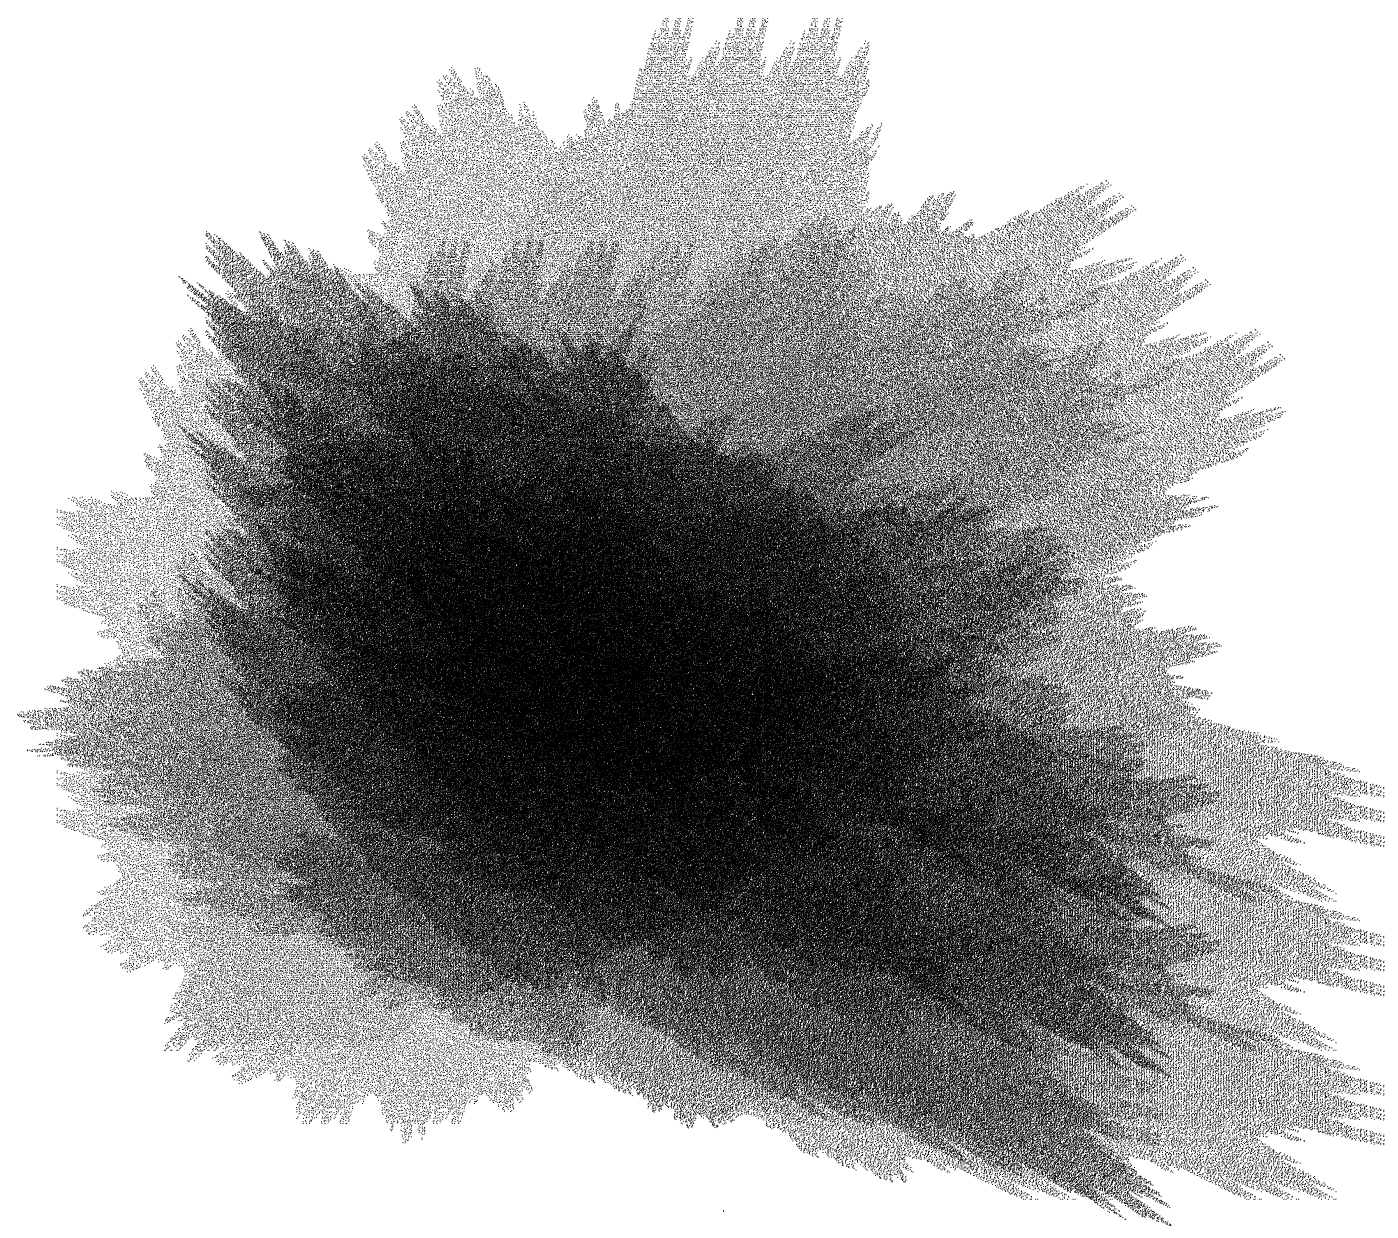
\includegraphics[width=15cm,keepaspectratio]{./graphics/leaf.png}\\
{\tiny \hspace*{\fill} \copyright{} Thomas Mejstrik}
\vspace{1cm}
}

\author{Thomas Mejstrik}

%\address{Fakultät für Mathematik, Universität Wien, Oskar-Morgenstern-Platz 1, 1090 Wien (Austria)}

\begin{document}

\maketitle

\tableofcontents

% !TeX encoding = UTF-8 Unicode
% !TeX root = manual.tex
% !TeX spellcheck = en_GB


\chapter{Introduction}
These packages provide functions for the computation of the joint spectral radius of a finite set of matrices using the modified invariant polytope algorithm
as well as functions for the work with multiple, multivariate, stationary subdivision schemes.
Some functions work also for symbolic matrices/subdivision schemes.

\section{System requirements}

In order to use the packages, you need at least Matlab R2016b.

The \texttt{sequence}- and the \texttt{subdivision}-package depend on the Matlab \texttt{Symbolic Math Toolbox} and the  
\texttt{Signal Processing Toolbox} but also run without the latter.
The \texttt{sequence}- and the \texttt{tjsr}-package depend on the Matlab \texttt{Parallel Computing Toolbox} but should run without it.
If these toolboxes are not installed, they can be installed as described in the Matlab documentation.

All other external, necessary toolboxes and functions are included in this package. These are
the \emph{TTEST}s~test-suite~v0.3, the \emph{SeDuMi} solver~v1.32 and the \emph{JSR-Toolbox}~v1.2b.

\section{Installation}
In order to install the \texttt{t}-packages do the following steps:

\begin{enumerate}

\item This package works with the \emph{Gurobi} solver and the Matlab \verb|linprog| solver, despite much slower with the latter since some optimizations of the modified invariant polytope algorithm are not possible to be realized with \verb|linprog|.

\item If you have not installed the \emph{Gurobi} solver yet and you want to use it, 
you should install it.
As of March~2019, the installation works as follows for academic users:
\begin{itemize}\label{install_gurobi}
    \item Download the Gurobi solver from 
    \href{http://www.gurobi.com/}{{\itshape http://www.gurobi.com/}} and
    extract the archive in a folder of your choice. 
    Do not choose a path which has blanks, i.e.\ instead of e.g.\ \texttt{/Gurobi 8/} use \texttt{/Gurobi\_8/}.
    
    \item Obtain a free academic licence. For that, open a shell, and execute in the
    \texttt{bin} subdirectory where you extracted the \texttt{Gurobi} files 
    the command which you find on the Gurobi page under the link 
    \emph{Free Academic License}. 
    The command looks like this 
    "\texttt{grbgetkey 1eb9501e-4e90-13e2-a19f-02e454bb2c50}".
    
    If this command fails, add "\texttt{./}" in front of the command, 
    i.e.\ instead of the above command, type 
    "\texttt{./grbgetkey 1eb9501e-4c91-11e9-a19f-02e454ff9c50}"
    If this command still fails, make sure you are connected to your universities network.
    
    If you are asked questions during the exectution of the command, always use the proposed default values, i.e.\ just press \emph{Enter}.
    
    \item At last, in Matlab run \verb|gurobi_setup| and \verb|savepath| afterwards.
        
\end{itemize}

\item \label{install_copy}
Copy the content of this archive 
(i.e.\ the folders \verb|TTEST| and \verb|ttoolboxes|)
into the directory of your choice.
In Matlab run the file \verb|setupt|, in the folder \texttt{ttoolboxes}.
This file adds all packages to the Matlab path and runs a self-test of all included functions.
If the test fails, you may run 
\texttt{runtests('testcell')},
\texttt{runtests('testdouble')},
\texttt{runtests('testm')},
\texttt{runtests('testsequence')},
\texttt{\justify runtests('testsubdivison')},
\texttt{runtests('testtjsr')},
\texttt{runtests('testtmisc')} or
\texttt{runtests('testTTEST')}
to test the individual packages.
\end{enumerate}

The Toolbox has been tested on several architectures (Windows, Linux, Mac) 
and Matlab versions (R2016b, R2017a, R2017b, R2018a, R2018b, R2019a).
If you encounter any problem, please contact the author at 
\begin{center}
\href{mailto:tommsch@gmx.at}{tommsch@gmx.at}.
\end{center}


%%%%%%%%%%%%%%%%%%%
% EOF
%%%%%%%%%%%%%%%%%%%

% !TeX encoding = UTF-8 Unicode
% !TeX root = manual.tex
% !TeX spellcheck = en_GB

\chapter{Changelog}

\section*{v1.0.7.2}
\begin{itemize}
\item Code changed to Python indentation style
\item version: v1.0.7.1: No error messages if Gurobi is missing
\item Minor changes due to Version R2019a.
\item Rewrote the test-suites. They now are in the standard Matlab script-based unit tests format, but need the \texttt{TTEST}-packages (also included in the package now) in order to work.
\item Fixed a bug in \verb|leadingeigenvector|.
\end{itemize}


\section*{v1.0.6}
\begin{itemize}
\item Made all warning texts to be Matlab warnings. The warning-id's are subject to be changed.
\item Rewrote \verb|findsmp|, making it faster and added the possibility to search for \emph{spectral minimizing products}.
Old implementation is renamed to \verb|findsmpold|.
\item Added options \verb|expect| and $\verb|expecte|$ to check parameters parsed by \verb|parsem|
\item Behaviour change in \verb|removezero|. Row vectors are now considered to be 2-dimensional arrays.
\item Colour options handling of \verb|plotm| improved.
\item Function \verb|tjsr_domain| is nearly finished. Its function name will be changed in a future release.
\item Added using of hyper-spherical coordinates to \verb|cart2sphm|
\item Bugfix in type \verb|3| of \verb|leadingeigenvector|
\item Behaviour change of option \verb|cycle| of \verb|leadingeigenvector|
\item Behaviour change of function \verb|tgenNecklaces|. 
Function now returns \emph{short} $n$-bead necklaces with $k$ colours instead
$n$-bead necklaces with $k$ colours instead.

\end{itemize}

\section*{v1.0.5}
\begin{itemize}
\item Added options \verb|noprint|, \verb|once|, \verb|save| and \verb|load| to \verb|vprintf|.
\item Added options \verb|link| and \verb|equal| to \verb|plotm|
\item Added type \verb|3| to \verb|leadingeigenvector|
\end{itemize}

% !TeX encoding = UTF-8 Unicode
% !TeX root = manual.tex
% !TeX spellcheck = en_GB


\chapter{Overview over the included packages}
This is the documentation for the most important functions of the packages
\texttt{cell}, \texttt{double}, \texttt{m}, \texttt{sequence}, \texttt{subdivision}, \texttt{tjsr} and \texttt{tmisc} (summarized as the \texttt{t}-packages).
The documentation for all functions (including those in this manual) can be read with the Matlab-command 
\texttt{help name}, where \texttt{name} is the name of a function, e.g.\ \texttt{help tjsr}. 

This file should also contain a copy of the \texttt{TTEST} package, which is necessary to run the test suites.

The \texttt{t}-packages can be downloaded from the Matlab file exchange
\href{https://de.mathworks.com/matlabcentral/fileexchange/}{\texttt{mathworks.com/matlabcentral/fileexchange}}.

\section{Naming/calling conventions and data-format}
\begin{itemize}
\item Most functions expect vectors in column format, contrary to Matlab's default. I.e. if you want the two column vectors 
$\left[\begin{array}{c c c}1&2&3\end{array}\right]^T$,
$\left[\begin{array}{c c c}7&8&9\end{array}\right]^T$
written in one matrix, all of the packages function expect them as%
\footnote{Internally most of the functions also use this data-format. 
Since sparse arrays in Matlab do not work well with this data-format, 
in a future release the function \texttt{tjsr} may change its data-format 
to Matlab's default.}
\begin{equation*}
\left[\begin{array}{c c c}1&7\\2&8\\3&9\end{array}\right].
\end{equation*}


\item All of the functions use \emph{name-value} pairs to pass options, e.g. \texttt{tjsr(...,'plot','norm')}, where \texttt{'plot'} is a \emph{name} and \texttt{'norm'} is a \emph{value}.
Some names expect no value, in which case the value can be omitted or given. 
If used without a value or with the value $1$ the option is enabled, if used with the value $0$, the option is disabled. 
Other arguments behind options which do not expect a value lead to undefined behaviour.

\item Optional arguments are written inside of square brackets in this documentation, with the exception when they are \emph{Options}, i.e.\ all options are optional.

\item All function-names/names/values/etc.\ are singular and written in lower-case, with the only exception when a corresponding mathematical symbol uses an upper-case letter.

\item Since Matlab (nearly) has no types for variables, we denote parameters which shall be whole numbers with the type \texttt{integer}, even if they are \texttt{double}s in reality.

\item The variables \texttt{idx} and \texttt{val} in the source-code are used only locally. They are only valid for some lines of code. They are re-used, since Matlab has no scope for variables.

\item The letters $\texttt{XX}$ in the source-code, indicates things which should be changed.
\end{itemize}

\section{Test-drivers}
Apart from the described example-usages in this documentation and in the \text{help} of each function, 
one can call the functions
\texttt{runtests('testcell')},
\texttt{runtests('testdouble')},
\texttt{runtests('testm')},
\texttt{runtests('testsequence')},
\texttt{runtests('testsubdivision')},
\texttt{runtests('testtjsr')} and
\texttt{runtests('testtmisc')}
which test every function included in the packages. 
By calling \texttt{INIT('all',1)} before executing a test suite, 
more tests are made when running the above commands.
The function \texttt{setupt} is a wrapper function, calling each of the functions above.
It succeeded on the following architectures (i.e.\ the \texttt{t}-packages are expected to run on the following architectures):
\begin{itemize}
\item Intel Core i5-4670S@3.8GHz, 8GB RAM\\
Linux 4.15.0-38,
Ubuntu 16.04.5 LTS\\
Matlab R2017a\\
with and without Gurobi v8.0.1

\item Intel Xeon IvyBridge-Ep E5-2650v2@2.6GHz, 64GB RAM\\
Linux 3.10.0, CentOS Linux 7\\
Matlab R2016b/R2017b/R2018b\\
with and without Gurobi v7.5.1/Gurobi v8.0.1

\item 
Intel Core i5-760@2.8GHz, 8GB RAM,\\
Windows 7 SP1\\
Matlab R2017a/R2018a\\
with and without Gurobi v8.0.1

\item
Intel Core i7@2.5GHz, 16GB RAM\\
OSX 10.10.5 (Yosemite), macOS 10.14.1 (Mojave)\\
Matlab R2017b\\
Gurobi v8.0.1

\item 
AMD Ryzen 5 3600, 32GB RAM,\\
Windows 10 LTSC, version 1809\\
Matlab R2018a\\
Gurobi v8.1.1

\item 
Intel Core i7-8650U@1.90GHz\\
Linux 4.15.0-99, Ubuntu 18.04\\
Matlab R2019a\\
without Gurobi
\end{itemize}
The packages do not run on Matlab versions before and including R2015b.

\section{\texttt{cell}-package}
This package implements functions for scalar operations on cell arrays. 
This package is not needed for any other package and does not depend on any other package.
\subsection*{Dependencies/Collisions}
It is possible that functions in this package are replaced by Matlab functions in future releases of Matlab.

\subsection*{Functions}
So far the following functions have been implemented:

Functions in the packages \texttt{cell} and \texttt{double} are likely to be replaced by Matlab functions in future releases of Matlab.
\texttt{diag},
\texttt{double},
\texttt{ldivide},
\texttt{minus},
\texttt{plus},
\texttt{rdivide},
\texttt{times},
\texttt{triu},
\texttt{uminus},
\texttt{uplus}.

\section{\texttt{double}-package}
This package contains functions which Matlab did not implement for \texttt{double}s but did implement for \texttt{sym}s.
This package does not depend on any other package.

\subsection*{Dependencies/Collisions}
The function in this package are hopefully replaced by Matlab functions in future releases of Matlab.

\subsection*{Functions}
So far the following functions have been implemented:
\texttt{isAlways},
\texttt{simplify}.

\section{\texttt{m}-package}
This package implements functions which generalize Matlab functions to $n$-arrays for arbitrary $n\in\NN_0$, 
and equips them with a consistent behaviour and interface.
Mathematical functions which are defined for an arbitrary number of arguments, 
but Matlab only accepts a small number (usually two), are also included in this package.
All functions should have the same input/output format as the original Matlab functions;
at least for basic inputs. Most of the functions do not rely on other packages. 

\subsection*{Dependencies/Collisions}
This package depends on the \texttt{sequence}-package and on the \texttt{tmisc}-package, but partly runs also without them.

{\color{red}
Some names of functions of this package may collide with functions from the
Matlab \texttt{Mapping Toolbox}, in particular \texttt{plotm} and \texttt{sizem}.
There are also reports that the function name \texttt{flatten} collides with some unknown package.}

The functions in this package are likely to be moved into a seperate namespace in future releases.

The function in this package are hopefully replaced by Matlab functions in future releases of Matlab.

\subsection*{Functions}
So far the following functions have been implemented:
\texttt{allm},  
\texttt{anym},  
\texttt{cart2sphm},
\texttt{convm},  
\texttt{dec2basem},  
\texttt{factorialm},  
\texttt{gcdm},  
\texttt{ind2subm},  
\texttt{isvectorm},  
\texttt{kronm},  
\texttt{lcmm},  
\texttt{maxm},  
\texttt{minm},  
\texttt{nchoosekm},
\texttt{ndimsm},  
\texttt{onesm}, 
\texttt{parsem}, 
\texttt{repmatm}, 
\texttt{sizem},  
\texttt{sph2cartm},  
\texttt{squeezem},
\texttt{summ},  
\texttt{upsamplem},  
\texttt{zerosm},  


The package also includes a small set of functions, originally not included in Matlab. These are:
\begin{param}
\item[sph2cartm2] Transforms hyperspherical to Cartesian coordinates, assuming the radius is one.
\item[cart2sphm2]Transforms Cartesian to hyperspherical coordinates, but does not return the radius.
\item[parsem] Parses \texttt{varargin}, similar to Matlab's \texttt{parse}\footnote{Most functions in the other packages rely on that function, thus it is included here.}.
\item[plotm] Unified interface for the visualization of various data types.
\item[repcellm] Works like \texttt{repmat} but returns cell-arrays.
\item[padarraym] Works like \texttt{padarray} from the \texttt{Image processing toolbox}, but works also for cell arrays, etc..\footnote{Written by~Notlikethat, \href{stackoverflow.com/users/3156750/notlikethat}{stackoverflow.com/users/3156750/notlikethat}, (2014) published under Common Creative Licence CC BY-SA.},
\end{param}



\section{\texttt{sequence}-package}
This package implements the vector space $\ell_0(\ZZ^s)$, $s\in\NN$.
The design-goal is, that \texttt{sequence}s behave exactly as arrays (whenever it makes sense) and code written for arrays can be used without modifications for \texttt{sequence}s. Unfortunately, direct referencing is not implemented yet. 

\subsection*{Dependencies}
The package depends on the \texttt{tmisc} and \texttt{m}-package. 

The package furthermore depends on the Matlab \texttt{Symbolic Math Toolbox}.
and uses functions from the Matlab \texttt{Signal Processing Toolbox} but also runs without the latter.

\subsection*{Functions}

So far the following functions are implemented:
\texttt{characteristic}   ($\chi$), 
\texttt{diffsequence}   ($\tilde{\nabla}_\mu$, $\nabla^k$), 
\texttt{norm} ($\|\vardot\|_p$), 
\texttt{supp} ($\operatorname{supp}$), 
\texttt{symbol} (the corresponding symbol),
\texttt{upsample} ($\uparrow_M$),
\texttt{conv} ($\ast$),
\texttt{nnz},
\texttt{ndims},
\texttt{size},
\texttt{ref},
and all point-wise operations. 


\section{\texttt{subdivision}-package}
This package implements functions for the work with subdivision schemes. Most of them can be used as a black-box.

\subsubsection*{Dependencies}
The package depends on the \texttt{m}-, \texttt{tmisc}- and \texttt{sequence}-package.
The package furthermore depends on the Matlab
\texttt{Parallel Toolbox} and \texttt{Symbolic Math Toolbox}.
Furthmore it uses functions from the Matlab \texttt{Signal Processing Toolbox} but also runs without the latter.

\subsubsection*{Important functions}
\begin{param}
\item[blf] Plots the basic limit function of a multiple subdivision scheme.
\item[constructOmega] Constructs the set $\Omega_C$ of a multiple subdivision scheme~\cite{CM18}.    
\item[constructordering] Constructs the data-type \texttt{ordering}.
\item[constructVt] Constructs a basis for the space $\tilde{V}_k(\Omega)$~\cite{CM18}.
\item[dimVVt] Computes the dimension of the spaces $V_k(\Omega)$ and $\tilde{V}_k(\Omega)$~\cite{CM18}.
\item[getS] Returns subdivision operators in this packages format.
\item[num2ordering] Computes number expansions for multiple multivariate number systems.
\item[ordering2num] Computes numbers corresponding for multivariate multiple number systems.
\item[restrictmatrix] Restricts matrices to a subspace.
\item[tile] Plots the attractor of a multiple subdivision scheme.
\item[transitionmatrix] Constructs transition matrices.
\end{param}

\subsubsection{Remaining functions}
\begin{param}
\item[characteristic] Returns the characteristic function of an index set.
\item[compresscoordinates] Returns an array representing the graph of a function.
\item[constructdigit] Constructs the usual digit set $M[0,1)^s\cap \ZZ^s$. 
\item[constructU] Constructs a basis for the space $U$~\cite{CP17}.
\item[constructVt] Constructs a basis for the space $\tilde{V}_k(\Omega)$~\cite{CM18}.
\item[daubechiesmask] Returns the mask coefficients for Daubechies' wavelet.
\item[findperiod] Searches for periodics in sequences.
\item[isodering] Determines if input is {ordering}.
\item[isS] Determines if input are {subdivision operator}s.
\item[isT] Determines if input are transition matrices.
\item[multiplyS] Concatenates subdivision operators.
\item[mask2symbol] Computes the symbol of a mask.
\item[normalizeS] Normalizes the values of a mask.
\item[ordering2vector] Converts an ordering to a vector of certain length.
\item[peter] Removes randomly columns of arrays.
\item[supp] Computes the support of a mask.
\item[symbol2mask] Computes the masks from given symbols.
\item[checktile] Tests if an attractor is a tile.
\item[tilearea] Tests heuristically if an attractor is a tile (for dimension $1$ and $2$).
\item[vector2ordering] Wrapper function for \texttt{findperiod}.
\end{param}



\section{\texttt{tjsr}-package}\label{tjsr_package}
This package implements functions to compute the $\JSR$ using the modified invariant-polytope algorithm.

\subsection*{Dependencies}
The package depends on the \texttt{m}- and the \texttt{tmisc}-package and partly on the \texttt{subdivision}-package
but also runs without the latter.
The package furthermore depends on the \texttt{Gurobi}-Solver
and the Matlab \texttt{Parallel Toolbox}.

If the \texttt{Gurobi}-solver is not installed, Matlab-functions will be used as a fall-back 
and the algorithm runs magnitudes slower.
If the \texttt{Parallel Toolbox} is not installed, the algorithm will run single-threaded.

\subsection*{Important functions}
\begin{param}
\item[findsmp%
\footnote{Copyright for algorithm \texttt{'genetic'} by~\cite{BC11}.}%
]
\hyperref[findsmp]{\textuparrow}
Searches for s.m.p.-candidates using various algorithms.

\item[invariantsubspace%
\footnote{Copyright for algorithm \texttt{'perm'} and \texttt{'basis} by~\cite{Jung2014} under the 3-clause BSD License.}%
]%
\hyperref[invariantsubspace]{\textuparrow}
Searches for invariant subspaces of matrices using various algorithms.

\item[tgallery]%
\hyperref[tgallery]{\textuparrow}
Returns sets of matrices, mostly used for \texttt{tjsr}.

\item[tjsr]%
\hyperref[tjsr]{\textuparrow}
Computes the joint spectral radius.

\item[tjsr\_getpolytope]%
\hyperref[tjsr_getpolytope]{\textuparrow} Returns the constructed invariant polytope returned by \texttt{tjsr}.

\item[preprocessmatrix]%
\hyperref[preprocessmatrix]{\textuparrow} Simplifies sets of matrices while preserving its $\JSR$.

\end{param}

\subsection*{Remaining functions}
\begin{param}
%\item[addcombination] Constructs short cycles from long cycles.
\item[binarymatrix] Returns sets of binary matrices.
\item[blockjsr] Returns the JSR of block diagonal matrices, given the JSR of the blocks.
\item[codecapacity] Returns matrices whose JSR is related to their capacity, given forbidden differences.
\item[computepolytopenorm] Computes the Minkowski-norm.
\item[daubechiesmatrix\footnote{Copyright for algorithm \texttt{'jung'} by~\cite{Jung2014} under the 3-clause BSD License. Copyright for algorithm \texttt{'gugl'} by Nicola Guglielmi.}] Constructs matrices whose $\JSR$ is related to the Daubechies' wavelets regularity.
\item[estimatepolytopenorm] Estimates the Minkowski-norm.
\item[estimatejsr] Rough estimate of the $\JSR$.
\item[extravertex] Finds vertices such that given polytope has non-empty interior.
\item[chooseval] Selects highest values of a vector.
\item[findsmpold] The old implementation of \texttt{findsmp}%
\footnote{Copyright for algorithm \texttt{'genetic'} by~\cite{BC11}. Copyright for algorithm \texttt{'gripenberg'} by~\cite{Jung2014} under the 3-clause BSD License.}
 (version$\leq 1.0.5$)
\item[intersectinterval] Intersects intervals.
\item[leadingeigenvector] Returns all leading eigenvectors of a matrix.
\item[makeorderinggraph] Constructs the graph corresponding to a partially ordered set.
\item[paritionatepolytope] Partitions points in $\RR^s$ into clusters of nearby points.
\item[reducelength] Removes periodics and cycles vectors such that they have smallest lexicographic value.
\item[removecombination] Constructs a minimal set of cycles.
\end{param}

\subsection*{Functions taken from others}
\begin{param}
\item[tavailable\_memory\footnote{\label{footnote_jsrtoolbox}Taken from \texttt{The JSR-toolbox}~\cite{Jung2014}. Published under the 3-clause BSD License.}] Returns the available memory.
\item[tbuildproduct\_fast\footnote{Uses code from~\cite{Jung2014}. Copyright: 3-clause BSD License.}] Constructs the product of matrices corresponding to a ordering.
\item[tcellDivide\footnoteref{footnote_jsrtoolbox}] Divides matrices in a cell.
\item[tgenNecklaces\footnoteref{footnote_jsrtoolbox}] Generation of all necklaces.
\item[tgraphSCC\footnoteref{footnote_jsrtoolbox}] Finds the strongly connected components of graph.
\item[tjointTriangul\footnoteref{footnote_jsrtoolbox}] Searches for invariant subspaces of matrices.
\item[tjsr\_zeroJsr\footnoteref{footnote_jsrtoolbox}] Decides if the JSR of a set of matrices is equal to zero.
\item[tliftproduct\footnoteref{footnote_jsrtoolbox}] Computes all products of matrices of a given length.
\item[tliftsemidefinite\footnoteref{footnote_jsrtoolbox}] Computes semi-definite liftings of matrices.
\item[tpermtriangual\footnoteref{footnote_jsrtoolbox}] Searches for invariant subspaces of matrices.
\end{param}

\noindent
All functions with prefix \texttt{tjsr\_} are subroutines of \texttt{tjsr} and are not documented here, since they are subject to big changes, whenever the main function \texttt{tjsr} is changed.
 


\section{\texttt{tmisc}-package}\label{tmisc_package}
This package contains useful functions. Most other packages rely on this package.

\subsubsection*{Dependencies}
The package depends on the~\texttt{m}-package and the~\texttt{double}-package.

\subsubsection*{Important functions}
\begin{param}
\item[findperiod] Searches for periodics of digit sequences.
\item[grCenter] Finds the centre of a tree.
\item[grVerCover] Computes all locally minimal vertex-covers of a graph.
\item[intersectspace\footnote{Copyright by Ondrej Sluciak, ondrej.sluciak@nt.tuwien.ac.at  under the 2-clause BSD License.}] Finds a basis of the intersection of subspaces.
\item[mixvector\footnote{Uses code from Jos van der Geest, samelinoa@gmail.com, under the 2-clause BSD License.}] Constructs all possible combinations of a set i.e.\ the Cartesian product.
\item[normalize] Normalizes matrices in various ways.
\item[removezeros] Deletes zeros in arrays in various ways.
\item[repcell] Repeats copies of an array.
\item[rho\footnoteref{footnote_jsrtoolbox}] Computes the spectral radius of matrices.
\item[searchincellarray] Searches in cell arrays. 
\item[setplus] Element-wise addition of vectors.
\item[setupt] Performs a self-test of all described packages.
\item[tbuildProduct\footnote{Uses code from~\cite{Jung2014}. Copyright: 3-clause BSD License.}] Constructs the product of matrices corresponding to an ordering.
\item[trho] Computes the spectral radius of matrices.
\item[uniquecell] Same behaviour as \texttt{unique}, but for cell-arrays.
\item[vdisp\footnote{\label{footnote_vdisp}Uses code by Stefan, University of Copenhagen,  under the 2-clause BSD License.}] Compact (but sometimes ugly) display of (nested) objects.
\item[vprintf] Powerful version of \texttt{sprintf} with the additional specifier \texttt{\%v}.
\end{param}

\subsubsection*{Remaining functions}
\begin{param}
    \item[cprintf\footnote{Copyright by Yair Altman (2015) under the 2-clause BSD License.}] Displays styled formatted text in the command window.
    \item[flatten] Converts nested cell arrays to flat cell arrays.
    \item[identifymatrix] Returns standard properties of matrices.
    \item[issquare] Tests if an array is a (hyper)-square.
    \item[issym] Tests if an object is symbolic.
    \item[iswholenumber] Tests if an array contains only whole numbers.
    \item[limsup] Computes the (cumulative) $\limsup$ of vectors.
    \item[liminf] Computes the (cumulative) $\liminf$ of vectors.
    \item[lexicographic] Orders vectors in a norm-lexicographic ordering.
    \item[nestedcellfun] Wrapper function calling \texttt{cellfun} for each cell in a (nested) (cell-)array.
    \item[makepositive] Multiplies arrays such that its first non-zero entry is positive.    
    \item[mat] Converts a vector to a matrix
    \item[nondiag] Extracts non-diagonal parts of 2-arrays and 2-cells.
    \item[num2color] Assigns colours to integers.
    \item[savetocellarray] Stores values in a cell array corresponding to a linear index-vector.
    \item[subsco] Indexing of matrices by coordinate-vectors.
    \item[tif] Ternary if operator.
    \item[unflatten] Converts a flat cell array to a nested cell array.
    \item[vec] Converts a matrix to a vector
   
\end{param}



%%%%%%%%%%%%%%%%%%%
% EOF
%%%%%%%%%%%%%%%%%%%


% !TeX encoding = UTF-8 Unicode
% !TeX root = manual.tex
% !TeX spellcheck = en_GB


\chapter{\texttt{m}-package}

\section{\texttt{plotm}}\label{plotm}
This function is a wrapper function to various graphics functions of Matlab.


% plotm( data, [options])
% Wrapper function which calls stem/plot/plot3 depending on the dimension of varargin{1}
% Also handles interval data
%
% Input:
%   data        dim x N array
%   [options]   everything which can be parsed by plot/plot2/plot3
%               if dim=1, stem is called instead of plot
%
% Options:
%   'box',val               Plots the hypercube of dimension val with volume 1
%   'rotate',val            (experimental) Rotates the current plot by 360 degree in steps of val degree.
%
% Options for 1-dim:
%   'height',val            scalar or 1x2 vector, default=[0 1],
%                           determines the length of the lines to be plotted
%                               scalar: Line goes from 0 to val
%                               vector: Line goes from val(1) to val(2) 
%
% Options for 2-dim:
%       'hull'              Plots also the convex hull
%       'boundary',val      (experminental) Plots also the boundary 
%                               val<= 1: computed with boundary
%                               val>1: points which have less neighbours are computed
%
% Options for 3-dim:
%       'contour'           Plots contour lines
%       'resolution',val    scalar, default depends on the input
%                           determines the resolution
%                               If val==0, the points are plotted
%                               otherwise val determines the resolution of the interpolated grid
%
% Info:
%   1-dim data:
%       Each point is plotted as a dot at height 1. 
%       The height can be changed by Option <'height',val>
%       To change the marker, the option <'Marker','something'> should be used
%
%   2-dim/3-dim data 
%       A point cloud is plotted
%
% E.g.: clf; hold on; clear all; load trimesh3d; plotm([x y z]','resolution',500); plotm([x y z]','resolution',0); view(3); plotm('rotate',0);
%       plotm(randn(2,40),'.-')
%       plotm(randn(1,40),'height',4);
%
% See also: surfm, plot, plot3, stem
%
% Written by: tommsch, 2016

% XX Write plotm4, using the commented out code below
% XX make plotm plot sequences
% XX hull for 3d plot

\subsection*{Syntax}
\begin{param}
    \item[{plotm( data, [options])}]
\end{param}

\subsection*{Input}
\begin{param}
    \item[data] One of the following:
    \begin{param}
        \item[dim x N vector] where $\texttt{dim}=1,2,3$.
        \item[sequence]
        \item[cell array of 1x2 vectors]
    \end{param}
\end{param}

\subsection*{Options}
\begin{param}

\item['box',int]        Plots the hypercube of dimension \texttt{int} with volume 1
\item['rotate',double]  Rotates the current plot by 360 degree in steps of \texttt{rotate} degrees.
\item[\textbullet] Most Matlab options which are passed as \emph{Name-Value} pairs should work, 
in particular Matlab linespecs.
\end{param}

\subsubsection*{Options for 1-dimensional plot}
\begin{param}
\item['height',val]     scalar or $1\times 2$ vector, \defval{\texttt{[0,1]}}\\
                        Determines the length of the lines to be plotted.
    \begin{param}                        
    \item[scalar] Line goes from 0 to \text{val}
    \item[vector] Line goes from \text{val(1)} to \texttt{val(2)}
    \end{param}                        
\end{param}

\subsubsection*{Options for 2-dimensional plot}
\begin{param}                        
   
\item['hull']              Plots the convex hull
\item['boundary',val]      scalar, \defval{\texttt{[]}}\\
                           Plots the boundary 
    \begin{param}
    \item[val>0]           Boundary is computed using a Delaunay triangulation
    \item[-1<=val<=0]      Boundary is computed with the Matlab function "boundary"
    \item[-inf<val<-1]     only points near the boundary are plotted    
    \end{param}                               

\end{param}

\subsubsection*{Options for 3-dimensional plot}
If no option of the ones below are given, the algorithm decides by itself what to plot.
\begin{param}      

\item['resolution',val]    scalar, \defval{depends on the input}
                           Determines the resolution
\begin{param}                           
       \item[0]      The points are plotted
       \item[scalar] Determines the resolution of the interpolated grid
\end{param}        
\item['contour']           Plots contour lines
\item['surface']           Plots a surface
\item['point']             Plots a point cloud
\end{param}

\subsection*{Example Usage}
\begin{param}
\item[{plotm(randn(1,40))}] 
\item[{hold on; plotm(randn(2,40),'.-','box',2)}]
\item[{plotm(randn(3,40),'resolution',0,'MarkerSize',100)}]
\item[{hold on; plotm(randn(3,40),'resolution',100,'surface','contour'); view(3);}]
\item[{plotm({[1 2];[4 6];[7 8]})}]
\item[{plotm(sequence(randn(20),[0;0]),'rotate',10)}]
\item[{plotm(sequence(randn(20,1),[0]))}]
\end{param}

\subsection*{Note}
\begin{itemize}
    \item More options may be added, and some options may be removed in the future.
\end{itemize}


\section{\texttt{parsem}}\label{parsem}
This function is meant to parse \texttt{varargin}.


%%%%%%%%%%%%%%%%%%%
% EOF
%%%%%%%%%%%%%%%%%%%

% !TeX encoding = UTF-8 Unicode
% !TeX root = manual.tex
% !TeX spellcheck = en_GB


\chapter{\texttt{subdivision}-package}

\section{\texttt{constructordering}}\label{constructordering}
The ordering in which the subdivision operators are applied for multiple subdivision schemes, is defined by the ``data-type'' \emph{ordering}. 
An ordering is a representation of an infinite periodic sequence.\footnote{Thus the multiple subdivision schemes defined by this package can be seen as stationary schemes.}
It is stored as an 1x2 - cell array, where the first cell is the non-periodic part, and the second cell is the periodic part.
Each cell can have an arbitrary number of rows.

The function \texttt{constructordering} takes vectors representing the non-periodic parts and the periodic parts of an ordering and returns it as a cell array.

\subsection*{Syntax}
\begin{param}
\item[{[ oo ] = constructordering( oo1, [pp1, oo2, pp2, ... ])}]
\end{param}

\subsection*{Input}
\begin{param}
    \item[oo1] vector of numbers, mandatory\\ The non-periodic part of the first row.
    \item[pp1] vector of numbers, optional\\ The periodic part of the first row.
    \item[ooi/ppi] vector of numbers, optional\\ The non-periodic/periodic part of the \texttt{i}$^{th}$ row.  
\end{param}

\subsection*{Output}
\begin{param}
    \item[oo] ordering\\The ordering defined by the input arguments. 
\end{param}

\subsection*{Note}
\begin{itemize}
    \item If \texttt{oo1} is an ordering, \texttt{oo1} is returned unchanged.
    \item All periodic and non-periodic parts must have the same length.
    \item The number of arguments is either 1 or an even number.
\end{itemize}

\subsection*{Example Usage}
\begin{itemize}
    \item \texttt{constructordering([1 2],[3 3])} returns \texttt{\{[1 2],[3 3]\}} which corresponds to the infinite sequence
    $1,2,3,3,3,3\ldots$.
    \item The number $\frac{1}{3}$ could be represented by \texttt{constructordering([],[3])}. Since \emph{ordering}s do not encode a decimal point, this sequence could also stand for the number $3.333\cdots$, etc..
\end{itemize}

\section{\texttt{getS}}
This function returns a finite set of \emph{subdivision operators}. This is a cell array, each row describing one subdivision operator. Each row has the entries
\begin{center}
    \texttt{\{ mask a, dilation M, digit-set D, ..., name n\}}.
\end{center}
The variables are: 
\begin{param}
    \item[mask a] $dim$-array\\Mask $a$ of the subdivision operator. 
    
    Note that univariate subdivision schemes have column vectors as masks.
    
    \item[dilation M] $dim\times dim$ matrix\\Dilation matrix $M$ of the subdivision operator.
    \item[digit-set D] $dim\times |\det M|$ matrix\\Set of representatives $D\simeq \ZZ^s/M\ZZ^s$.
    \item[name n] string\\Name of the subdivision operator.
\end{param} 
In future releases of the package, data-fields may be added to subdivision-operators. The \texttt{name} will always be the last entry in each row.

The function \texttt{getS} returns examples of \emph{subdivision operator}s in the described format.

\subsection*{Syntax}
\begin{param}
\item[{[ S ] = getS(dim || cellarray || name || list, [options])}]
\end{param}

\subsection*{Input}
\begin{param}
    \item[dim] integer\\
    Returns all subdivision operators encoded in the file \texttt{getS} in the section \texttt{\%UNNAMED OPERATORS} of the source file \texttt{getS}.
    E.g.: \texttt{getS(2);}
    
    \item[cellarray] cell-array \texttt{\{[a],M,[D],[n]\}} where \texttt{a}, \texttt{M}, \texttt{D}, \texttt{n} are described above.\\
    Takes a subdivision operator (or parts from it) and computes the missing variables. Only \texttt{M} is mandatory and thus the cell array must be at least of size $1\times2$.
    
    If \texttt{D} is not given, $D:=M\ZZ^{dim}\cap\ZZ^{dim}$.\\
    If \texttt{a} is not given $a:=\chi_D$, where $\chi$ is the characteristic function.\\
    If \texttt{n} is not given $n:=\texttt{'unnamed'}$.
    
    E.g.: \texttt{getS(\{[0.5 1 0.5]',2\});}
    
    
    \item[name] string\\
    Returns the subdivision operator with name \texttt{name} encoded in the file \texttt{getS} in the sub-routine \texttt{getS\_named}.
    
    E.g.: \texttt{getS('1\_Hassan\_Dodgson\_3point');}
    
    \item[list] name-value pairs of strings\\
    The possible names are 
    \texttt{'a'} or \texttt{'mask'}, 
    \texttt{'M'} or \texttt{'dilation}, 
    \texttt{'D'} or \texttt{'digit'}, 
    \texttt{'n'} or \texttt{'name'}.
    The possible values are as described above.
    
    E.g.: \texttt{getS('a',[.25 .5 .25;.5 1 .5;.25 .5 .25],'M',[2 0; 0 2],'n','tensorlinear');}    
\end{param}

\subsection*{Options}
\begin{param}
    \item['bigcheck'] Enables some data-integrity checks.

    \item['characteristic']  Instead of the masks, the characteristic function of the digit sets is returned as the masks.
    
    \item['help'] The strings of the named subdivision operators (i.e.\ the allowed strings for \texttt{name})  are printed (among some other strings)\footnote{This is actually an option for the function \texttt{parsem}.}.    

    \item['Omega'] Instead of the digit sets, the support of the masks minus the digit sets is returned as the digit sets.
    
    \item['nocheck'] Disables basic data-integrity checks.

    \item['supp'] Instead of the digit sets, the support of the masks is returned as the digit sets.        

    \item['verbose',val] integer, \defval{1}\\Verbose level.

\end{param}

\subsection*{Output}
\begin{param}
\item[S] cell array of subdivision operator(s)
\end{param}   

\subsection*{Note}
\begin{itemize}
\item All subdivision operators in a cell array should be for the same dimension.
\item Matlab versions prior to R2018a cannot display subdivision operators for dimension 1, and throw an error if attempted to do so. 
\end{itemize}

\subsection{Subset of the possible values for \texttt{name}}

\subsubsection{Univariate schemes}
\begin{param}    
\item['1\_all'] All named subdivision schemes of dimension $1$.
\item['1\_rand'] A random subdivision scheme of dimension $1$.
\item['1\_4point'] The 4-point scheme {\small$a=\frac{1}{16}\tbmatrix{-1&0&9&16&9&0&-1}$}, $M=2$.
\item['1\_DD'] The Dubuc-Deslauriers scheme {\small $a\!=\!\frac{1}{256}\tbmatrix{3& \!0& \!-25& \!0 &\!150 &\!256& \!150& \!0 &\!-25&\!0 &\!3}$}, $M\!=\!2$.
\item['1\_balanced\_ternary'] The balanced ternary number system $M=3$, $D=\{-1,\ 0,\ 1\}$.
\item['1\_cantor'] A scheme whose attractor is the Cantor-set.
\item['1\_daubechies',n] The $n^{th}$ Daubechies wavelet scaling function.
\item['1\_devil\_stairs'] A subdivision scheme whose basic limit function is the devil-stairs function.
\item['1\_Hassan\_Dodgson\_3point'] The Hassan-Dodgson 3-point scheme {\small$a\!=\!\frac{1}{16}\tbmatrix{1&\!\!5&\!\!10&\!\!10&\!\!5&\!\!1}$}, $M\!=\!3$.
\item['1\_spline\_binary-2'] The second order B-Spline scheme.
\item['1\_strange\_interpolatory'] An interpolatory scheme which does not fulfil $a(0)=1$.
\item['1\_three\_disjoint\_Om'] A scheme which has three disjoint invariant sets $\Omega$~\cite{CM18}.
\end{param}



\subsubsection{Bivariate schemes}
\begin{param}
\item['2\_all'] All named subdivision schemes of dimension $2$.
\item['2\_rand'] A random subdivision scheme of dimension $2$.
\item['2\_butterfly'] The butterfly scheme.
\item['2\_flash'] Scheme whose attractor is the flash.
\item['2\_McLure'] Non-integer scheme with self affine 4-tile.
\item['2\_rqj43'] Example from~\cite[Example 4.3]{CJR2002}.
\item['2\_sierp'] A scheme whose attractor is the Sierpinski triangle.
\item['2\_twindragon'] Scheme whose attractor is the twindragon.
\item['2\_V0neqV0bar\_1'] Scheme where $V_0\neq\tilde{V}_0$~\cite{CM18}.
%\item['2\_superomega'] Scheme whose super-tile is the cover-image.
\end{param}


\subsubsection{Trivariate schemes}
\begin{param}
\item['3\_rand'] Returns a random subdivision scheme of dimension $3$.
\end{param}

\subsubsection{Quadrovariate schemes}
\begin{param}
\item['4\_rand'] Returns a random subdivision scheme of dimension $4$.
\item['4\_cex\_Pot97'] Dilation matrix which does not posses a digit set, such that the corresponding attractor is a tile~\cite{Pot97}.
\end{param}


\subsection*{Example Usage}
\begin{param}
\item[getS(2)] Returns all unnamed subdivision operators of dimension $2$. The returned set may be empty, if there are no unnamed subdivision operators.
\item[getS('2\_butterfly')] Returns the butterfly scheme.
\item[getS('1\_all')] Returns all named subdivision operator of dimension 1.
\item[{getS('a',[.25 .5 .25;.5 1 .5;.25 .5 .25],'M',[2 0; 0 2],'n','tensorlinear');}] The first bivariate tensor-product B-spline.
\end{param}


\section{\texttt{blf}}
This function plots the basic limit function of multiple subdivision schemes.
    
\subsection*{Syntax}
\begin{param}
\item[{[ c, PM, xyzv, oo ] = blf( [oo], S, [options] )}]
\end{param}

\subsection*{Input}
\begin{param}
\item[{[oo]}] ordering, optional\\
Defines the ordering in which the subdivision operators are applied.
If \texttt{oo} is not given, a random ordering is computed.
\item[S] subdivision operators (or something else), mandatory\\
The parameter \texttt{S} is passed to \texttt{getS} and the returned value is used.
\end{param}

\subsection*{Options}

% Options:
\begin{param}

\item['diff',val]                  $1 \times dim$-vector or integer, \defval{0}\\
    Computes (partial) derivatives (finite differences). If \texttt{diff} is a vector the given partial derivative is computed. 
    If \texttt{diff} is a scalar, then all partial derivatives of that order are computed.
    


\item['iteration',val]             integer, \defval{depends on \texttt{S}}\\
                                   Computation stops after \texttt{iteration} many iterations.

\item['maxiteration',val]          integer, \defval{50}\\ Maximum number of iterations.

\item['maxnumpoint',val]           integer, \defval{30000}\\ Maximum number of points in the output-sequence to be computed.

\item['numpoint',val]              integer, \defval{30000}\\ Number of points in the output-sequence to be computed.

\item['plot',cellarray]            cell array or scalar, \defval{\texttt{\{\}}}\\
                                   Arguments passed to \texttt{plotm}.
                                   If $\texttt{plot}=0$, nothing is plotted.\\
                                   E.g.\ \texttt{'plot',\{'Color','red'\}}.

\item['start']                     $dim$-array, \defval{$\delta_0$}\\ Starting sequence.

\item['verbose',val]               integer, \defval{1}\\Verbose level.

\end{param}

\subsection*{Output}
\begin{param}
\item[c] $dim$-array or cell array of $dim$-arrays.\\
Iterated sequence, i.e.\ $\texttt{c}=
S_{\texttt{oo}_\texttt{n}}
\cdots
S_{\texttt{oo}_\texttt{2}}
S_{\texttt{oo}_\texttt{1}}
(\texttt{start})$.    
If \texttt{diff} is given and there is more then one partial derivative, \texttt{c} is a cell array.

\item[PM] $dim\times dim$ matrix\\Dilation matrix corresponding to the returned mesh.\\
{\color{red} There is a bug, and the returned matrix may be the transposed.}

\item[xyzv] $dim + 1 \times N$ matrix\\
Column vectors $v$ containing the function values at the position $xyz\in\RR^{dim}$.

\item[oo] vector\\ Ordering used. Equals (input-)\texttt{oo} if given.
\end{param}

\subsection*{Example Usage}
\begin{param}
\item[{[ c, PM, xyzv ,So ] = blf( '2\_butterfly', 'iteration',3, 'diff',1 )}]
\end{param}

\section{\texttt{tile}}
Plots the attractor corresponding to a multiple subdivision scheme. I.e.\ for given \texttt{S} and \texttt{oo}, the set defined by
\begin{equation*}
\texttt{M}_{\texttt{oo}_1}^{-1}\texttt{D}_{\texttt{oo}_1}+
\texttt{M}_{\texttt{oo}_1}^{-1}\texttt{M}_{\texttt{oo}_{2}}^{-1}\texttt{D}_{\texttt{oo}_2}+
\texttt{M}_{\texttt{oo}_1}^{-1}\texttt{M}_{\texttt{oo}_{2}}^{-1}\texttt{M}_{\texttt{oo}_{3}}^{-1}\texttt{D}_{\texttt{oo}_3}+
\cdots.
\end{equation*}

\subsection*{Syntax}
\begin{param}
\item[{[ Q, oo ] = tile( [oo], S, [options] )}]
\end{param}

\subsection*{Input}
\begin{param}
\item[{[oo]}] ordering, optional\\
The ordering in which the subdivision operators are applied
\item[S] subdivision operators, mandatory\\
The subdivision operators
\end{param}

\subsection*{Options}
\begin{param}
\item['digit']                    \defval{false}\\Computes iterated digit sets instead of the attractor.

\item['iteration',val]             integer, \defval{depends on \texttt{S}}\\
Computation stops after \texttt{iteration} many iterations.

\item['maxiteration',val]          integer, \defval{50}\\Maximum number of iterations.

\item['numpoint',val]              integer, \defval{30000}\\Number of points in the output-sequence to be computed.

\item['plot',cellarray]            cell array or scalar, \defval{\texttt{\{\}}}\\
Arguments passed to \texttt{plotm}, e.g.\ \texttt{\{'Color','red'\}}.
If $\texttt{plot}=0$, nothing is plotted.

\item['round',val]                integer or $1\times 2$-vector, \defval{\texttt{1e-2, 1e-12}}\\
If \texttt{round} is an integer, the same round value is used in each iteration.
If \texttt{round} is a vector, the round values are linearly interpolated.

\item['start',array]              $dim$-array, \defval{$\delta_0$}\\The starting set.

\item['supertile',n]              integer\\Computes the supertile $K=\cup_{j}(M_j^{-1}K+D_j)$ instead of the attractor. 

\item['verbose',val]              integer, \defval{1}\\Verbose level.

\end{param}

\subsection*{Output}
\begin{param}
\item[Q] $dim\times N$ matrix\\The computed attractor.
\item[oo] vector\\Ordering used. Equals \texttt{oo} (Input) if given.
\end{param}
    
\subsection*{Example Usage}
\begin{param}
\item[{tile('2\_frayed\_squares','round',[.1 1e-2])}]
\item[{tile('1\_cantor','digit')}]
\item[{tile([getS('2\_rand'); getS('2\_rand')],'supertile','iteration',10)}]   
\end{param} 

\section{\texttt{constructOmega}}
Constructs the set $\Omega_C$ as described in~\cite{CM18}.

\subsection*{Syntax}
\begin{param}
    \item[{[ Om ] = constructOmega( S, [options] )}]
\end{param}

\subsection*{Input}
\begin{param}
    \item[S] cell array of subdivision operators, mandatory
\end{param}

\subsection*{Options}
\begin{param}
    \item['lexicographic']      \defval{false}\\Orders the output set lexicographically.
    \item['Omega',val] matrix, optional, \defval{automatically computed}\\
        Starting set. If not given, a point is computed where to start from.
        In some cases, the algorithm may not find a good starting point, and the returned set is not minimal.
    \item['stable'] \defval{false}\\Does not order the set the output set.        
    \item['verbose',val] integer, \defval{1}\\Verbose level.
\end{param}    

\subsection*{Output}
\begin{param}
    \item[Om] matrix\\The set $\Omega_C$.
\end{param}

\subsection*{Example Usage}
\begin{param}
    \item[{constructOmega('2\_butterfly','Omega',[2;2],'stable')}]
\end{param}   

\subsection{Basic implementation}
\begin{lstlisting}
function [ Om ] = constructOmega( S, Om )
% S: cell array of subdivision schemes. Each row consists of a, M and D.
% Om: (Optional) the starting set
% Ex: a=1/3*[1 2 3 2 1]; M1=[2 -1;1 -2]; M2=[1 1;1 -2]; D=[0 1 2;0 0 0];
%     constructOmega({a, M1, D; a, M2, D})
    a=S(:,1); M=S(:,2); D=S(:,3);                  %extract the sets a,M and D
    J=numel(a);                                    %number of subdivision operators
    dim=size(M{1},1);                              %the dimension
    if(nargin==1); Om=zeros(dim,1); end            %if Omega is not given, set it to zero
    while(true)
        sizebefore=size(Om,2);                     %used to check if elements were added 
        for j=1:J                                  %iterate through all subdiv. operators
            OmN=M{j}\setplus(supp(a{j},dim),Om,-D{j}); %compute new possible entries
            OmN=round(OmN(:,sum(abs(OmN-round(OmN)),1)<.5/abs(det(M{j})))); %round to integers
            Om=unique([Om OmN]','rows')';          %remove duplicates
        end
        if(size(Om,2)==sizebefore); break; end     %if no elements were added, terminate
    end
    
function [ X ] = setplus( varargin )
% setplus(A,B) = { x=a+b : a in A, b in B}, operates column wise
% Ex: setplus([1 2; 1 0],[0 -1;-1 -1]); %Output: [0 1 1 2;0 -1 0 -1]
    sze=size(varargin,2);                 %number of sets
    X=varargin{sze};                      %the output set
    for i=sze-1:-1:1                      %iterate through all sets
        A=varargin{i};                    %the set to be added
        X=repmat(A,1,size(X,2))+reshape(repmat(X,size(A,2),1),size(A,1),[]); %add the set
        X=unique(X','rows')';             %remove duplicates
    end
    
function [ L ] = supp( a, dim )
% returns the support of an array. First entry is supposed to have index (0,0,...,0)
% Ex: supp([1 1;0 1],2) %Output: [0 0 1;0 1 1];
    L=zeros(dim,nnz(a));                  %output variable
    CO=cell(1,dim);                       %dummy-variable to do calculation with indices
    j=1;                                  %index-variable for the columns of D
    for i=1:numel(a)                      %iterate through all elements of the masks
        if(a(i)~=0)                       %if the element is nonzero, save the indices
            [CO{:}]=ind2sub(size(a),i);   %get the indices
            L(:,j)=[CO{:}]'-1;            %add converted cell to vector
            j=j+1;                        %increase counter
        end
    end
\end{lstlisting}
 

\section{\texttt{constructVt}}
Constructs a basis for the space $\tilde{V}_k(\Omega)$, as described in~\cite{CM18}.

\subsection*{Syntax}
\begin{param}
\item[{[ V, Om, Xmuf ] = constructVt( Om, [k] , [options])}]
\end{param}

\subsection*{Input}
\begin{param}
\item[Om] $dim \times N$ array of column vectors, mandatory\\
The set for which $V_k$ shall be constructed
\item[{[k]}] integer or a vector of integers greater equal zero, optional\\
Index or indices $k$.

\end{param}

\subsection*{Options}
\begin{param}
    \item['01'] Allows to give input \texttt{Om} as a logical array.\\ 
    E.g.\ \texttt{constructV( [1 0; 1 1; 1 0], 0, '01','verbose',2)} is equivalent to \texttt{constructV( [0 0; 1 0; 1 1; 2 0]' , 0,'verbose',2)}.
    
    \item['verbose',val] integer, \defval{1}\\Verbose level.
    
\end{param}

\subsection*{Output}
\begin{param}
    \item[Vt] matrix (or cell array of matrices) of column vectors.\\
    The basis (bases) for the space $\tilde{V}_k$.
    If $k$ is empty, then all spaces $\tilde{V}_k$ are computed for which $\dim \tilde{V}_k>0$.
    \item[{[Om]}] array of column vector\\The set for which $\tilde{V}_k$ is constructed.
    \item[{[Xmuf]}] scalar/vector\\ 
    If set, all sets $X_\mu$ of the corresponding space $V_k$ are non-empty, see~\cite{Mej19}.    
\end{param}

\subsection*{Note}
\begin{itemize}
    \item The functions \texttt{constructV} and \texttt{constructU} construct the spaces ${V}_k(\Omega)$ and $U_k(S)$ as described in~\cite{CM18}. They have nearly the same interface as \texttt{constructVt}, so they are not described in this manual. See the \texttt{help} of these functions for more informations.
    
    \item If one wants to use the matrix-approach for the characterization of convergence of subdivision schemes, the set $\Omega$ has to fulfil two assumptions. $(i)$ $\dim \tilde{V}_k(\Omega)=\dim V_k(\Omega)$, $(ii)$ $X_\mu(\Omega)$ is non-empty for all $|\mu|=k+1$. The function \texttt{dimVVt} may be used to check these two conditions.    
    
\end{itemize}

\subsection*{Example Usage}
\begin{param}
    \item[{Om=constructOmega('2\_butterfly'); constructV(Om,1)}]
\end{param}
% Output:
%   V           matrix/or cell array of matrices, each column is one basis vector for the space V_i i \in k
%
% E.g.: vdisp(constructVt([0 1 2 3]))
%       Om=constructOmega('2_butterfly'); constructV(Om,1)
%       constructV([1 0 1; 0 1 1; 1 0 1],1,'01')
%
% See also: constructVt, constructU
%
% Reference:
%   Set V_k is described in:
%       Maria Charina, Thomas Mejstrik,
%       Multiple multivariate subdivision schemes: Matrix and operator approaches, 
%       Journal of Computational and Applied Mathematics, 2018

\section{\texttt{restrictmatrix}}
Restricts matrices to a subspace and checks whether the subspace is invariant or not, 
i.e.\ with the notation from below, the function computes 
\begin{equation}
\texttt{TT}=
\left[\begin{array}{c c}\texttt{TA}&\ast\\\texttt{NULL}&\texttt{TR}\end{array}\right]=
\texttt{BASIS}^{-1}\cdot\texttt{T}\cdot\texttt{BASIS}.
\end{equation}
\subsection*{Syntax}
\begin{param}
\item[{[ TA, TT, TR, NULL, BASIS ] = restrictmatrix( T, A, [options] )}]
\end{param}

\subsection*{Input}
\begin{param}
\item[T] square matrix or cell array of square matrices, mandatory\\
The matrices which shall be restricted to the subspace \texttt{A}.
\item[A] rectangular matrix, mandatory\\
Matrix defining the subspace using column vectors.
\end{param}


\subsection*{Options}
\begin{param}

\item['epsilon',val] double, \defval{$10^{-12}$}\\The matrices are considered to be invariant if all norms of the residua \texttt{NULL\{i\}} are less then $dim\cdot\texttt{epsilon}$.

\item['smallsize'] Removes all columns of \texttt{A} (starting from the last column), without changing the rank of \texttt{A}, before computing the restriction.

\item['verbose',val] integer, \defval{1}\\ Verbose level
\end{param}
\subsection*{Output}
If the input \texttt{T} is a cell array, then the outputs 
\texttt{TA}, 
\texttt{TT}, 
\texttt{TR} and 
\texttt{NULL}
are also cell arrays. \texttt{BASIS} is always a matrix.
\begin{param}
\item[TA] $dim_A\times dim_A$ matrix (or cell array of)\\ Restriction of \texttt{T} to \texttt{A}
\item[TT] $dim_T\times dim_T$ matrix (or cell array of)\\ \texttt{T} in the basis of \texttt{A} complemented to a basis of $\RR^{dim_T}$.
\item[TR] $dim_{T-A}\times dim_{T-A}$-matrix (or cell array of)\\ Lower right corner of matrix \texttt{TT}.
\item[NULL] $dim_{T-A}\times dim_{A}$-matrix (or cell array of)\\ Lower left corner of \texttt{TT}. If \texttt{T} is \texttt{A} invariant, then \texttt{NULL} consists of zeros only.
\item[BASIS] $dim_T\times dim_T$ matrix (or cell array of)\\Complemented basis of \texttt{A} to a basis of $\RR^{dim_T}$.
\end{param} 

\subsection*{Example Usage}
\begin{param}
\item[{restrictmatrix([1 1 0; 0 1 1; 1 0 1],[1 -1 0; 0 1 -1]')}]
\end{param}

\section{\texttt{transitionmatrix}}
Constructs transition matrices 
$T_{d, \Omega}=(\texttt{a}(\alpha-\texttt{M}\beta+d))_{\alpha, \beta\in\Omega}$ 
where 
$\texttt{a}\in\texttt{S}$ are subdivision masks, 
$M\in\texttt{S}$ are dilation matrices, 
$d\in\texttt{D}\in\texttt{S}$, $D\simeq\ZZ^s/\texttt{M}\ZZ^s$, are digit sets and $\Omega\subseteq\ZZ^s$ is an invariant set for these matrices~\cite{CM18}.
\subsection*{Syntax}
\begin{param}
\item[{[ T, Om, Vt ] = transitionmatrix( S, [options] )}]
\end{param}

\subsection*{Input}
\begin{param}
\item[S] cell array of subdivision operators, mandatory
\end{param}

\subsection*{Options}
\begin{param}
\item['colsum',val]  double, \defval{disabled}\\
Tests if the columns sum up to \texttt{colsum}. If \texttt{colsum==0}, the column-sum of the first column of the first transition matrix in \texttt{T} is used.

\item['infindices']        Entries of indices not element of the support of the masks, are replaced by $\infty$ instead of $0$.

\item['noflat']            Function returns cell array of cell arrays, each corresponding to one subdivision operator.

\item['onlyindices'] Function returns $(dim+\#\Omega) \times \#\Omega$ matrix with the indices used for construction of the transition matrices (instead of the values of the mask \texttt{a} at the indices position).

\item['Omega',val] $dim\times N$ integer matrix, \defval{automatically constructed using \texttt{constructOmega}}\\
Index set used for construction of the transition matrices.

\item['verbose',val] integer, \defval{1}\\Verbose level.

\item['V',val] integer, \defval{1}, {\color{red}experimental}\\ Constructs set $\Omega$ such that $X_\mu$ is non-empty for all $|\mu|<\texttt{val}+1$, see [Mejstrik, PhD Thesis, 2019]. This option is needed if one wants to compute whether a subdivision scheme is $C^\texttt{val}$.
\end{param}

\subsection*{Output}
\begin{param}
\item[T] cell array of matrices\\The transition matrices.
\item[Om] The set $\Omega$ used to compute the transition matrices.
\item[Vt] matrix, only returned if $\texttt{'V',val}$ is given\\
The difference space $\tilde{V}_\texttt{val}$.
\end{param}

\subsection*{Example Usage}
\begin{param}
\item[{vdisp(transitionmatrix({1/4*[1 4 3]',2}))}]
\end{param}

\section{Example showing how to use the \texttt{subdivision}-package}

\begin{example}\label{ex_subdivision}
This example computes the Hölder regularity of the stationary subdivision scheme given by the subdivision operator 
$S=(a,M)$, 
with mask $a=\frac{1}{4}\left[\begin{array}{cccc}1 & 1& 3&3\end{array}\right]$ 
and dilation $M=2$.
We first generate the cell array of subdivision operators
\begin{verbatim}
S=getS('a',1/4*[1;1;3;3],'M',2);
   %There is a bug in Matlab which throws an error for the command disp(S). 
   %Thus the semi-colon is important.
\end{verbatim}
To plot the basic limit function we call
\begin{verbatim}
blf(S);
\end{verbatim}
We next construct the transition matrices and restrict them to the invariant subspace $V_0$. 
We also construct the space $\tilde{V}_0$. To apply the joint spectral radius approach to compute the regularity of subdivision-schemes, the dimension of $V_0(\Omega)$ and $\tilde{V}_0(\Omega)$ must coincide.
\begin{verbatim}
[T, Om]=transitionmatrix(S); %compute transition matrices and the set Omega
plotm(Om,'x') %plot the set Omega
V0=constructV(Om,0)                   %Construct space orthogonal to polynomial sequences
V0bar=constructVt(Om,0);            %Construct space of differences of delta
if(size(V0,2)~=size(V0bar,2)); 
    fprintf('Set Omega is wrong.');   %Test ifV0==V0bar
end
TV0=restrictmatrix(T,V0); vdisp(TV0); %restrict transition matrices and display them
\end{verbatim}
The last step is to compute the Hölder regularity using the modified invariant polytope algorithm.
\begin{verbatim}
[JSR, type]=tjsr(TV0);  
al=-log(JSR)/log(2) %Hoelder regularity. The 2 comes from the dilation M=2.
\end{verbatim}

\end{example}

%%%%%%%%%%%%%%%%%%%
% EOF
%%%%%%%%%%%%%%%%%%%

% !TeX encoding = UTF-8 Unicode
% !TeX root = manual.tex
% !TeX spellcheck = en_GB


\chapter{\texttt{tjsr}-package}


\section{\texttt{findsmp}}\label{findsmp}
This function searches for 
spectral maximizing and spectral minimizing products\footnote{s.min.p's are experimental}, 
in the following s.m.p.-candidates.
Two algorithm types available: \emph{Gripenberg type algorithms} and the \emph{Genetic algorithm}.

\subsection*{Syntax}
\begin{param}
\item 
\texttt{[ cand, nearlycand, info ] = findsmp( T, [algorithm], ['smaxp'|'sminp'], [options] )}
\end{param}

\subsection*{Input}
\begin{param}
\item[T] cell array of square matrices of the same size, mandatory\\The input matrices.
\item[{[algorithm]}] string, \defval{\texttt{'modgrip'}}\\ 
Algorithm to use:
\begin{param}
    \item['gripenberg'/'grip'] Standard Gripenberg's algorithm~\cite{Grip96}, does not miss candidates.
    
    \item['lowgripenberg'/'lowgrip']  Modified Gripenberg algorithm keeping small products.

    \item['highgripenberg'/'highgrip'] Modified Gripenberg algorithm keeping large products.
    
    \item['modifiedgripenberg'/'modgrip'] Modified Gripenberg algorithm  keeping small and large products.
    
    \item['randomgripenberg'/'randgrip'] Modified Gripenberg algorithm randomly keeping products
    
    \item['bruteforce','bf'] Brute force algorithm computing every possible product.
    This is the only algorithm which is proven to work for searching s.min.p's.
    
    \item['necklacebruteforce'/'nlbf'] Brute force algorithm computing every possible product which is a short necklace%
    \footnote{A string is a \emph{short necklace} if it is not power of a shorter necklace.}.
    
    \item['genetic'] Genetic algorithm~\cite{BC11}. Fast algorithm to compute lower bounds of the $\JSR$.
    \end{param}
\end{param}

\subsection{Options for Gripenberg type algorithm}
One can use either pre-defined options corresponding to one specific algorithm, and/or set all/any options by hand.

\begin{param}
\item['vpa']                           Tries to convert input to \texttt{vpa} prior computing
   \item['double']                        Tries to convert input to \texttt{double} prior computing
   \item['verbose',val]                   \defval{1}, Defines the verbose level. 
   \item['nosimplify']                    Does not simplify products \texttt{cand} and \texttt{nearlycand}
   \item['maxtime',val]                   \defval{\texttt{inf}}, Maximal time used for computation
   \item['maxeval',val]                   \defval{\texttt{inf}}, Maximum number of evaluations (approximate)
   \item['bound',val]                     \defval{\texttt{[]}}, Searches until 
    \begin{itemize}
    \item  the bounds of the joint/lower spectral radius is in $(\texttt{val(1)}, \texttt{val(2)})$; or
    \item  it is proven that the bounds cannot be fulfilled anymore.
    \end{itemize}

   \item['nearlycandidate',val]           \defval{0.99}, experimental, Nearlycandidates must have spectral radius larger than val*jsrbound(1),
   \item['shortnearlycandidate',val]      \defval{1}, Removes all nearlycandidates whose ordering is longer than the val*maximal-length-of-candidates-ordering.
                                          Note that 'genetic' algorithm does not search for nearly-candidates at the moment, thus this option has no effect for 'genetic' algorithm
   \item['maxsmpdepth',val]               maximal length of products which is searched for. Default value depends on algorithm used. Can be
    \begin{itemize}
    \item arbitrary high (>100) for \texttt{modgrip}, \texttt{lowgrip}, \texttt{highgrip}, \texttt{randgrip}, 
    \item high (<30) for \texttt{gripenberg},
    \item small (<12) for \texttt{bruteforce} and   
    \item small (<15) for \texttt{necklacebruteforce}.  
    \end{itemize}

\item['norm',h]           function handle, \defval{\texttt{@norm}, i.e. 2-norm}, handle to a norm function
\item['rho',h]			  function handle, \defval{\texttt{@rho}}, handle to a spectral radius function               
\item['delta',val]        double, \defval{depends on algorithm}, relative delta used in the Gripenberg Algorithm.
\item['N',val]            scalar or 1x3 vector of doubles, \defval{depends on algorithm}, number of kept products in each step
                                          \begin{itemize}
                                          \item \texttt{N(1)}  ... number of products with smallest matrix norm kept
                                          \item \texttt{N(2)}  ... number of products with largest matrix norm kept
                                          \item \texttt{N(3)}  ... number of products randomly kept
                                          \end{itemize}
\item['minsmpdepth',val]               double, \defval{1}, Minimal length of products
\item['nearlycanddelta',val]           double, \defval{0.99}, Maximal relative difference of spectral radius between candidates and nearly-candidates
\item['maxnumnearlycandidate',int]     integer, \defval{10}, Maximum number of nearly candidates returned. 
If number of nearly candidates is larger, \texttt{'nearlycanddelta'} is decreased

\item['sminp' | 'smaxp']               \defval{\texttt{'smaxp'}}, Defines whether to search for s.min.p's or s.max.p's.
Option \texttt{'sminp'} is experimental.
\item['hardworking',val]               double, \defval{1}, sets \texttt{'maxsmpdepth'} to $\texttt{'hardworking'} \times \text{length of last-smpcandidate}$
 each time a new candidate is found
\item['epsilon',val]                   double, \defval{1e-10}, epsilon used for comparing spectral radii
\end{param}

Pre-defined options:
\begin{param}
    \item['gripenberg'/'grip'] Standard Gripenberg's algorithm~\cite{Grip96}, does not miss candidates, \texttt{delta=0.95}.
    
    \item['lowgripenberg'/'lowgrip']  Modified Gripenberg algorithm keeping \texttt{N} small products, \texttt{delta=1}.

    \item['highgripenberg'/'highgrip'] Modified Gripenberg algorithm keeping \texttt{N} large products, \texttt{delta=1}.
    
    \item['modifiedgripenberg'/'modgrip'] (default) Modified Gripenberg algorithm  keeping \texttt{N/2} small and \texttt{N/2} large products, \texttt{delta=1}.
    
    \item['randomgripenberg'/'randgrip'] Modified Gripenberg algorithm keeping \texttt{N} random products, \texttt{delta=1}.
    
    \item['bruteforce','bf'] Brute force algorithm, computing every possible product.
    This is the only algorithm which is proven to work for searching s.min.p's.
    
    \item['necklacebruteforce'/'nlbf'] Brute force algorithm, computing every possible product which is a short necklace%
    \footnote{A string is a \emph{short necklace} if it is not power of a shorter necklace.}.
\end{param}

\subsection*{Output}
\begin{param}
\item[cand]         cell array of column vectors\\Ordering of the products with highest normalized spectral radius.
\item[nearlycand]   cell array of column vectors\\Orderings of products with nearly highest normalized spectral radius.
\item[info]         struct\\Additional info, depending on the used algorithm and options.  May contain the following fields:
    \begin{param}
    \item[info.time] double\\ Time in seconds needed for the computation.
    \item[info.jsrbound] 1x2 vector\\Bounds for the JSR/LSR.
    \item[info.spectralgap] double\\Relative difference between info.jsrbound and second biggest eigenvalue found (from nearly-candidates)
    \item[info.count] integer\\
    Approximate number of computed matrices.
    \end{param}
\end{param}

\subsection*{Note}
\begin{itemize}
\item The Gripenberg type algorithms are parallelised, the genetic algorithm is not.
\item All Gripenberg type algorithms return true lower and upper bounds for the $\JSR$/$\LSR$.
\item There is a bug in the Genetic algorithm and the returned upper bound for the $\JSR$ is sometimes wrongly normalized.
\item See the \texttt{help} of \texttt{findsmp} for the options for the genetic algorithm.
\end{itemize}

\subsection*{Example Usage}
\begin{param}
\item[{\texttt{[ c, nc, info ] = findsmp( {[1 -1; 3 -2], [1 3; -1 -1]}, 'maxsmpdepth', 15 )}}]
\item[{\texttt{[ c, nc, info ] = findsmp( {[1 -1; 3 -2], [1 3; -1 -1]}, 'gripenberg' )}}]
\end{param}

\subsection{Basic Implementation}
\begin{verbatim}
function [c] = gripenberg_modified( M, N, D )
%Tries to find smp-candidates in a fast way.
%Ex: gripenberg_modified( {[2 1; 0 -2],[2 1; -1 -2]}, 4, 10 )
J = length( M );  %number of matrices
o = 1:J;          %the orderings of the products to be checked
c = {};           %list of candidates
r = 0;            %lower bound for JSR
for d = 1:D                        %do D iterations
    NR = zeros( 2, size(o,2) );    %norm and rho of candidates
    for i = 1:size( o, 2 )         %can be parallelised using parfor!
        P = buildProduct( M, o(:,i) );                  %construct matrices
        NR(:,i) = [norm( P ); max( abs(eig(P)) )]; end; %compute norm and rho
    NR = NR.^(1/d);                %normalize norm and rho
    if r < max( NR(2,:) )          %test if new bound was found
        c = {};                    %delete candidates
        r = max( NR(2,:) ); end;   %update lower bound for JSR
    c = [c num2cell( o(:,NR(2,:) >= r), 1 )]; %add candidates to c
    idx = NR(1,:) < r;             %remove everything with norm less than JSR
    NR(:,idx) = []; 
    o(:,idx) = [];
    [NR,idx] = sortrows( NR' );    %sort correspdonding to norm
    NR = NR.'; 
    idx = idx.';
     nNR = size( NR, 2 ); 
    if nNR > 2*N                   %keep highest and lowest norms
        o = o(:,[idx(1:N) idx(nNR-N+1:nNR)]); 
    else                           %keep everything if N is too big
        o = o(:,idx); end;      

    o = [repmat( o, [1 J] );       %make new orderings of products    
         reshape( repmat(1:J,[size(o,2) 1]), 1, [] )];    end;

function M = buildProduct( A, prod )
% Constructs the product of matrices of A corresponding to prod.
M = eye( size(A{1},1) );
for t = 1:length( prod ); 
    M = A{prod(t)}*M; end
\end{verbatim}

\section{\texttt{tgallery}}\label{tgallery}
This function provides example-sets of matrices.
It is useful for testing algorithms and other purposes. 
It also makes use of Matlab's \texttt{gallery}.
\subsection*{Syntax}
\begin{param}
\item \texttt{[ val ] = tgallery( what, dim, N, k, [options] )}
\end{param}
\subsection*{Input}
\begin{param}
\item[what] string, mandatory\\Controls the return value.
\item[dim] integer, mandatory in most cases\\Dimension of matrices. In some cases 
\item[N] integer, mandatory in most cases\\Number of matrices.
\item[k] anything, mandatory in some cases\\Number of matrices.
\end{param}
The variables may have another meaning in some cases, as described below.
\subsection*{Options}

\begin{param}
\item['bool'] flag\\Returns boolean matrices.
\item['int'] flag\\Returns integer matrices.
\item['norm'] flag\\Returns matrices with 2-norm 1.
\item['pos'] flag\\Returns matrices with positive entries.
\item['rho'] flag\\Returns matrices with spectral radius 1.
\item['seed',val] integer or struct returned by \texttt{rng}, \defval{empty}\\Seed for random number generator. 
If \texttt{seed} is set, Matlab's random number generator has the same state before and after execution of the function.
\item['sparse',val] double, \defval{0}\\Returns sparse matrices
\item['verbose',val] integer, \defval{1}\\Verbose level.
\end{param}

\subsection*{Output}
\begin{param}
\item[val] cell array of square matrices\\The returned matrices.
\end{param}


\subsection*{Note}
Most options preserve do not preserve certain properties of the matrices, e.g.\ the entries in the matrix returned by
\texttt{tgallery('rand\_gauss',10,1,'pos')} are not normally distributed anymore.

\subsection{Possible values for \texttt{what} and their mandatory arguments}
This section lists a subset of the possible values for \texttt{what}, followed by the mandatory parameters. For example,
\begin{center}
\texttt{tgallery('rand\_pm1', 2, 1, 'seed', 10)}
\end{center}
 returns a cell array with one element, containing the $2\times2$ matrix
 \begin{equation*}
\left[\begin{array}{rr}
0& 0\\
1& -1\\
\end{array}\right].
 \end{equation*}
\subsubsection{Random matrices}
\begin{param}

\item['rand\_bool',dim,N] Random matrices with values 0, 1.
%\footnote{\label{footnote_boolpm1}\texttt{rand\_pm1} and %\texttt{rand\_bool} are good example to test the balancing of multiple trees of the invariant polytope algorithm.}
\item['rand\_doublestochastic',dim,N] Random double-stochastic matrices.
\item['rand\_doublestochastic\_neg',dim,N] Random double-stochastic matrices with pos.\ and neg.\ values.
%\item['rand\_colu\_0',dim,N] Random matrices with pos.\ entries, column-norm=1 and i.i.d.\ singular values. 
%\item['rand\_colu\_1',dim,N] Random matrices  with non-neg.\ entries, column-norm=1.
\item['rand\_corr\_1',dim,N] Random correlation matrices with pos.\ entries.
\item['rand\_corr\_0',dim,N] Random correlation matrices with non-neg.\ entries.
\item['rand',dim,N] Random matrices with equally distributed values in $[0,\ 1]$.
%\item['rand\_equal',dim,N] Random matrices with equally distributed values in $[-1,\ 1]$.
\item['rand\_gauss',dim,N] Random matrices with normally distributed values.
\item['rand\_hess',dim,N] Random orthogonal upper Hessenberg matrices.
\item['rand\_neg',dim,N] Random matrices with equally distributed values in $[-1,\ 1]$.
\item['rand\_normal',dim,N] Random matrices with normally distributed values.
%\item['rand\_orthog\_1'] Random orthogonal matrices with complex leading eigenvalue.
%\item['rand\_orthog\_2'] Random orthogonal matrices with complex dual leading eigenvalue.
\item['rand\_pm1',dim,N] Random matrices with values -1, 0, 1.%\footnoteref{footnote_boolpm1}
\item['rand\_stochastic',dim,N] Random column-stochastic matrices.
\item['rand\_stochastic\_neg',dim,N] Random column-stochastic matrices with positive and negative values.
\item['rand\_unitary',dim,N] Random unitary matrices.
\item['rand\_zero',dim,N] Random matrices with spectral radius 0.
\item['rand\_TU',dim,len] Transition matrices of a subdivision scheme in $\RR^\texttt{dim}$ with random dilation matrix and random mask with $\texttt{len}^\texttt{dim}$ non-zero entries, restricted to the subspace $U$ as defined in~\cite{CP17}.
\item['rand\_TV0', dim, len] Transition matrices of a subdivision scheme in $\RR^\texttt{dim}$ with random dilation matrix and random mask with $\texttt{len}^\texttt{dim}$ non-zero entries, restricted to the subspace $V_0$ as defined in~\cite{CM18}.

\end{param}

\subsubsection{Matrices from applications}
\begin{param}
\item['binary',dim,N,k] Matrices whose linear entries equals the number \texttt{k} in base 2. E.g.:  
\begin{equation*}
\texttt{tgallery('binary',2,2,19)}=
\left\{ 
\left[ \begin{array}{cc}0&0\\0&1\end{array} \right],\ 
\left[ \begin{array}{cc}0&1\\0&1\end{array} \right]
\right\},
\end{equation*}
since $19_{[10]}=00010011_{[2]}$.

If there exists $\tilde{\texttt{k}}<\texttt{k}$ such that the returned set for  $\tilde{\texttt{k}}$ would be the same, the function returns the empty set.
\item['binary2',dim,N,k] The same as \texttt{'binary'}, but if there exists $\tilde{\texttt{k}}<\texttt{k}$ such that the returned set for $\tilde{\texttt{k}}$ would have the same $\JSR$, the function may return the empty set.
\item['cex'] Pair of 2x2 matrices which has no s.m.p.~\cite{TB00}, returned approximately with 61 digits.
\item['code',C] (C is a cell array of row-vectors) Matrices whose $\JSR$ is related to the capacity of a code with forbidden differences \texttt{C}. See the source-code of \texttt{codecapacity} for more information. E.g.: 
\texttt{tgallery('code',\{[1 1 0 1]\})}.
\item['daub',dim] Matrices whose $\JSR$ is closely related to the Hölder-exponent of Daubechies' wavelets.
\item['euler',dim] Matrices in connection with the Euler partition function~\cite{GP13}.
\item['nondominant'] Set $\{ 
\left[\begin{array}{c c}1 & 1\\0& 1\end{array}\right],\  
\tfrac{4}{5}\left[\begin{array}{c c}1 & 1\\0& 1\end{array}\right]
\}$ with non-dominant s.m.p..
\end{param}

\subsubsection{Matrices from papers}
\begin{param}
\item['grip\_p45'] Matrices 
$\{
\left[\begin{array}{c c}0 & 1\\0& 0\end{array}\right],\  
\left[\begin{array}{c c}0 & 0\\1& 0\end{array}\right]
\}$ 
from~\cite[p.~45]{Grip96}.


\item['grip\_p52'] Matrices 
$\{
\frac{1}{5} \left[\begin{array}{c c}3 & 0\\1& 3\end{array}\right],\  
\frac{1}{5} \left[\begin{array}{c c}3 & -3\\0& -1\end{array}\right]
\}$ 
from~\cite[p.~52]{Grip96}. 


\item['morris\_p3'] Matrices 
$\{
\left[\begin{array}{c c}2 & 2\\0& 0\end{array}\right],\  
\left[\begin{array}{c c}1 & 1\\1& 1\end{array}\right]
\}$ 
from~\cite[p.~3]{Morris2010}.
\item['prot2012\_p35'] Example for the Pascal rhombus~\cite[p.~35]{GP13}.
\item['prot2012\_p40'] Example~\cite[p.~40]{GP13}.
\item['prot2012\_p43'] Example for the Euler binary problem~\cite[p.~43]{GP13}.
\item['prot2012\_p44'] Example for the Euler ternary problem~\cite[p.~44]{GP13}.
\item['prot2016'] Matrices for the subdivision scheme~\cite[p.~33, p.~35, p.~50]{GP13}.

\item['mejstrik\_119\'] Matrices $\mathcal{X}=
\{
\left[\!\begin{array}{r r}
\dfrac{15}{92} & \dfrac{-73}{79}\\[2.ex]
\dfrac{56}{59}  & \dfrac{89}{118}\end{array}\!\right]
,\
\left[\!\begin{array}{c c}
\dfrac{-231}{241} & \dfrac{-143}{219}\\[2.ex]
\dfrac{103}{153}  & \dfrac{-38}{65}\end{array}\!\right]
\}
$ with s.m.p.-length 119.

%\item['mejstrik\_119\_2'] Matrices
%\begin{align*}
%\mathcal{X}=
%\{
%&\left[\begin{array}{r r}
%\dfrac{2936824268245481}{18014398509481984} & \dfrac{-1040403609775579}{1125899906842624}\\[2.ex]
%\dfrac{8548815905856585}{9007199254740992}  & \dfrac{6793656059295549}{9007199254740992}\end{array}\right],\\
%&\left[\begin{array}{r r}
%\dfrac{-8633497502531381}{9007199254740992} & \dfrac{-2940665869269935}{4503599627370496}\\[2.ex]
%\dfrac{6063507393887449}{9007199254740992}  & \dfrac{-5266479768915639}{9007199254740992}\end{array}\right]
%\}
%\end{align*}
%with s.m.p.-length 119.

\item['mejstrik\_longsmp',x] Matrices $\tilde{\mathcal{C}}_x=\{ 
\left[\begin{array}{c c}1 & 1\\0& 1\end{array}\right],\  
\left[\begin{array}{c c}0 & 0\\x& 0\end{array}\right]
\}$ with s.m.p.-length approximately $e\cdot x$.

\end{param}

\subsection*{Example Usage}
\begin{param}
\item[{tgallery('rand\_gauss',5,2,100,'rho')}]
\item[{tgallery('mejstrik\_119')}]
\end{param}


\section{\texttt{invariantsubspace}}\label{invariantsubspace}
Searches for invariant subspaces of matrices $M\in\texttt{M}$, 
i.e.\ a change of basis $B$ such that all matrices $B^{-1}MB$, $M\in\texttt{M}$ have block-triangular form.
The function uses three different algorithms: \texttt{permTriangul}, \texttt{jointTriangul} from~\cite{Jung2014} and an implementation of~\cite{CP17}.
The returned matrices still may have invariant subspaces which can or cannot be found using this function.
\subsection*{Syntax}
\begin{param}
\item \texttt{[ Mret, B ] = invariantsubspace( M, ['type'], [options] )}
\end{param}

\subsection*{Input}
\begin{param}
\item[M] cell array of matrices, mandatory\\The matrices.
\item[{['type']}] string, \defval{\texttt{'auto'}}, optional
    \begin{param}
    \item['none']      Nothing happens,  \texttt{Mret=\{M\}}, \texttt{B=eye(dim)}.

    \item['perm']      Tries to find a permutation such that all $\texttt{M\{i\}}$ are in block-diagonal form.
    \item['basis']     Tries to find a basis such that all $\texttt{M\{i\}}$ are in block-diagonal form.
    \item['trans']     Tries to find subspaces generated by differences of basic limit functions as occurring in subdivision theory~\cite{CP17}. The algorithm first computes numerically, then symbolically, then using \texttt{vpa}.
    \item['auto']      (default) The algorithm tries \texttt{'perm'}, \texttt{'basis'} then \texttt{'trans'} (numerically).
    \end{param}

\end{param}
\subsection*{Options}
\begin{param}
\item['verbose',int] integer, \defval{1}\\Verbose level.
\end{param}
\subsection*{Output}
\begin{param}
\item[Mret]   cell array of matrices\\
                The blocks in the block diagonal of the matrices in basis \texttt{B}.
\item[B]      matrix\\Basis, i.e.\ \texttt{B\^{}(-1)*M\{i\}*B} has block-diagonal form.
\end{param}

\subsection*{Example Usage}
\begin{param}
\item[{\texttt{[ M, B ] = invariantsubspace( \{[1 0 ; 1 2], [3 -1; -1 3]\}, 'basis', 'verbose', 2 )}}]
\end{param}




\section{\texttt{tjsr}}\label{tjsr}
Computes the $\JSR$ of a set of square-matrices.
\subsection*{Syntax}
\begin{param}
\item \texttt{[ JSR, info, allinfo ] = tjsr( M, [options] ) }
\end{param}

\subsection*{Input}
\begin{param}
\item[M] Cell array of matrices, mandatory\\The input matrices whose $\JSR$ shall be computed.
\end{param}

\subsection{Important options}
This is a list of the most important options (which should be sufficient for the standard-user). In a later section all available options are listed.
\begin{param}


\item['balancingvector',val] vector, \defval{empty}\\If given, these numbers are used to balance the multiple cyclic trees. The vector must have as many entries as there are cyclic-roots (including extra-vertices). 

\item['delta',val] double, \defval{1}\\Accuracy. For $\texttt{delta}<1$ the algorithm is faster, but returns only bounds for the $\JSR$.

\item['invariantsubspace',string] string, \defval{\texttt{'auto'}}\\  \texttt{string} is one of the following:
\texttt{'none'}, \texttt{'perm'}, \texttt{'basis'}, \texttt{'trans'}, \texttt{'auto'}. See the documentation of \nameref{invariantsubspace} for more information.

\item['maxsmpdepth',int] integer, \defval{depends on the size and number of matrices}\\Maximal length of s.m.p.-candidates to search for.
    
\item['nearlycandidate',val] double, \defval{$\simeq0.9999$}\\Relative difference between s.m.p.-candidates and nearly-s.m.p.s spectral radii.
If you are sure that a certain s.m.p.-candidate is an s.m.p., 
but the algorithms returned intermediate bounds stuck on some level, try to play with the value of \text{nearlycandidate}.

\item['nobalancing',val] \defval{0}\\Disables balancing.

\item['ordering',cell] cell array of matrices of column vectors, \defval{empty}\\ Orderings of s.m.p.-candidates.    

\item['plot',string] string, \defval{\texttt{'none'}}
    \begin{param}
    \item['norm'] Plots intermediate norms
    \item['polytope'] Plots the constructed polytope
    \item['L'] Plots the number of vertices left to compute (at the moment)
    \end{param}


\item['proof'] \defval{false}\\Proofs the invariance of the polytope after termination of the algorithm and returns bounds for the $\JSR$ w.r.t.\ that polytope. The proof uses Matlab functions and is \emph{very} slow and may fail in some cases.




\item['verbose',val] integer, \defval{1}\\Verbose level. If $\texttt{verbose}<0$ the algorithm suppresses error-messages (not recommended!).
\end{param}


\subsection*{Note}
\begin{itemize}
\item The algorithm is parallelised and starts the default Matlab-pool if there is no pool available. If a special pool is needed (e.g. a non-local pool), it has to be started by the user beforehand.
\item The algorithm is split up into three main-functions, responsible for the following tasks:
\begin{itemize}
\item \texttt{tjsr}:
        Preprocessing the input;
        Starting the Matlab pool;
        Restarting the algorithm  with different parameters (if needed);
        Postprocessing the output.
\item \texttt{tjsr\_preworker}:
        Finding invariant subspaces;
        Starting \texttt{tjsr\_worker} for each subspace;
        Finding candidates;
        Balancing trees;
        Setting up the cyclic-root.   
\item \texttt{tjsr\_worker}:
        Computing the invariant polytope.
\end{itemize}
\item Most of the sub-routines of the algorithm are in separate files with the prefix \texttt{tjsr\_}. We do not described these functions here, since they are subject to big changes whenever the main function \texttt{tjsr} is changed. Nevertheless, most of them have a documentation inside of their source-code.
\end{itemize}

\subsection*{Output}
\subsubsection{Screen Output}
\emph{\color{red} Output written in red must be read.}
For some options or input matrices, the algorithm delivers wrong results and these messages warn in these cases.
These messages are printed again after the termination of the algorithm.

\paragraph{Output in front of the progress bar}
\begin{itemize}[noitemsep]
\item \texttt{Time: x/y}       Time needed for the last iteration/total time needed for building the tree.
\item \texttt{JSR = [ x, y ]}  Interval in which the JSR lies.
\item \texttt{norm = x}        Current minimal computed norm of the polytope.
\item \texttt{In: x, Out: y}   Number of points which lie inside or outside the polytope, checked by estimating the Minkowski-norm.
\item \texttt{\#test: x/y}      Number of points to test in this iteration/number of points to check in total
\item \texttt{\#V: x/y}         Number of points in simplified polytope/number of points in polytope in total
\item \texttt{'Test old vertex'}  Old vertices of polytope get estimated again.
\end{itemize}
\paragraph{Output in the progress-bar}
\begin{itemize}[noitemsep]
\item \texttt{i}  Vertex is proofed to be inside of the polytope, but norm is unknown
\item \texttt{x}  Vertex is proofed to be outside of the polytope, but norm is unknown
\item \texttt{\_}  Vertex is inside of the polytope
\item \texttt{.}  Vertex is machine-epsilon-near to the polytope 
\item \texttt{,}  Vertex is 1000*machine-epsilon-near to the polytope
\item \texttt{o}  Vertex is slightly outside
\item \texttt{O}  Vertex is far outside
\item \texttt{m}  Negative value occurred during computation of norm, vertex is added
\item \texttt{8}  Inf occurred during the computation of the norm, vertex is added
\item \texttt{?}  NaN or Inf occurred during the computation of the norm, vertex is added
\item \texttt{E}  Some error occurred during the computation of the norm, vertex is added
\end{itemize}

Verbose levels higher than 2 generate much more output, which is not described here.

\subsubsection{Data Output}
\begin{param}
\item[JSR] double or 1x2-vector.\\Interval containing the exact value for the $\JSR$ or an interval containing the $\JSR$.
\item[info] struct\\ Contains nearly all data which was generated during the computation. Most important fields are described here, all other fields are described below.
    \begin{param}
    \item[info.cyclictree.ordering]    cell array of matrices of column vectors\\
    All orderings used for the roots of the cyclic trees.
    
    \item[info.cyclictree.smpflag] vector\\
    Defines what the orderings are: $0$ : s.m.p.-candidate, $1$ : nearly-s.m.p, $2$ : extra-vertex.
    
    \item[info.cyclictree.V] cell array of matrices\\All generated vertices, each column is one vertex. To obtain the (invariant) polytope call\\
    \texttt{tjsr\_getpolytope(info)}
    
    \item[info.info.errortext] string\\All important error-messages.
    
    \item[info.JSR] double or 1x2-vector\\The same as \texttt{JSR}.
    \item[info.counter] struct\\Some self-explaining numbers.
    \item[info.block] cell array of structs, only returned if there are invariant subspaces\\
    If returned, each cell in \texttt{info.block} contains the \texttt{info}-struct for that block.
    The sub-structs \texttt{info.info} and \texttt{info.counter} contains aggregated informations from \texttt{info.block\{:\}}.
    \end{param}

\item[allinfo] cell array of structs\\
If the algorithm restarts, only the \texttt{info} struct of the very last run is returned (to save memory). All other \texttt{info}-structs are returned as the cell array \texttt{allinfo}.
\end{param}

\subsection{Example Usage}\label{tjsr_example_usage}
The algorithm (in the optimal case) does not need to be called with any parameters, i.e. a call of the form \texttt{tjsr(A)}, where \texttt{A} is the cell array of matrices whose $\JSR$ shall be computed, is sufficient.
Nevertheless, in some examples the algorithm does not work as expected and manual interaction is necessary.

For our examples in this section we make use of the function~\nameref{tgallery} which returns example matrices. Some options used for these examples are described in detail in Section~\ref{tjsr_alloptions}.
\begin{itemize} 

\item This example shows how to specify the cyclic-roots. 
We use for the example the set of matrices\\
\texttt{A=tgallery('rand\_pm1',3,2,'seed',100)}, i.e.\ 
$\texttt{A}=\{\texttt{A}_1,\texttt{A}_2\}$,
\begin{equation*}
\texttt{A}_1=\left[\begin{array}{rrr}
 1& 1& 1\\
 0& 1&-1\\
 1& -1&-1\\
\end{array}\right],
\quad
\texttt{A}_2=\left[\begin{array}{rrr}
 0& 0& 1\\
-1&-1& 0\\
 1& 1&-1\\
\end{array}\right].
\end{equation*}


The set $\texttt{A}$ has an s.m.p.\ $A_1 A_2^8$, which can be computed with \texttt{tjsr(A)}.

The command \texttt{tjsr(A,'ordering',\{[2]'\})} starts the algorithm with a wrong s.m.p.. The algorithm finds better s.m.p.-candidates and restarts several times. Note that automatic extra-vertices are disabled, if we specify an ordering.

If we want to add extra-vertices we can do it in two ways.
\begin{param}
\item[{tjsr(A,'extravertex',\{[.1 0 0]'\})}]~
\begin{itemize}
\item This command specifies only the extra-vertex. The s.m.p.-candidates and nearly-s.m.p.s are computed automatically.
\end{itemize}

\item[{tjsr(A,'ordering',\{[1 2 2 2 2 2 2 2 2]', []'\},'smpflag',[0 2],'v0',...\newline
\{[0.058585928823279  -0.687551547968790   0.723768303968635]', [.1 0 0]'\})}]~\\
 This command specifies vectors of the cyclic-roots. The downside is, that one needs to give the exact eigenvalues of all s.m.p.-candidates and nearly-s.m.p.s.
\begin{itemize}
\item The option \texttt{'smpflag',[0 2]} specifies that we want two cyclic-roots. The first is the root corresponding to an s.m.p.-candidate (number \texttt{0}), the second root corresponds to an extra-vertex (number \texttt{2}). If we also want to specify a root for a nearly-s.m.p., we have to use the number \texttt{1}.

\item The option \texttt{'v0',\{[0.05859  -0.68755   0.72377]' [.1 0 0]'\}} specifies the eigenvectors/vectors used to start the cyclic-root. They must be given as a cell array of column vectors.

\item If one also wants to specify the dual-leading eigenvectors, this has to be done using the option \texttt{'v0s'}.

\item The option \texttt{'ordering',\{[1 2 2 2 2 2 2 2 2]', []'\}} specifies the orderings of the cyclic-roots.
The first is the ordering of the s.m.p.. 

Note that $(i)$ \emph{orderings of extra-vertices MUST be empty},
$(ii)$ \emph{orderings MUST be given as column vectors}, and $(iii)$ are written in reversed polish notation, i.e.\ the ordering \texttt{1 2 3} is the product $\texttt{A}_3\texttt{A}_2\texttt{A}_1$.

If there is more than one ordering corresponding to a vector \texttt{v0}, it must be given as a matrix. 
E.g.: \texttt{'ordering',\{[1 2 2 2; 1 2 2 0]'\}} means that 
$\texttt{A}_2^3\texttt{A}_1 \texttt{v0}_1=\texttt{A}_2^2\texttt{A}_1 \texttt{v0}_1=\texttt{v0}_1$.
\end{itemize}



\end{param}

\item This example presents balancing, automatic extra-vertices and approximate computation options.
We use for the example the set of Daubechies-matrices 
\texttt{D7=tgallery('daub',7)}. 

\begin{param}

\item[{tjsr(D7)}] Just starting the algorithm computes that this set has two s.m.p.s: $\texttt{D7}_1$ and $\texttt{D7}_2$. 

\item[{tjsr(D7,'balancingvector',[1 1.02 .01 .01 .01 .01 .01])}] Uses the given balancing vector to balance the trees. This option is useful when one wants to prove the invariance of the invariant polytope by hand.

\item[{tjsr(D7,'nobalancing')}] This command disables the balancing (and the algorithm applied to this example will not terminate). Using verbose level to 4, \texttt{tjsr(D7,'nobalancing','verbose',4)}, we see that the third line of numbers does not stop to grow. This line corresponds to the number of added vertices to the third cyclic-tree.

\item[{tjsr(D7,'autoextravertex',0)}] This command disables the automatic extra-vertices. Since the polytope for these matrices is very flat, the LP-program fails to compute the Minkowski-norm and reports all vertices to be outside (This can be seen by the fact, the the computed norms are always $\infty$).

\item[{tjsr(D7,'nobalancing','delta',.99999)}] This command multiplies the matrices prior computing the cyclic-tree by $0.99999$. Thus the algorithm will terminate, although we did not balance the trees. Clearly, the returned value is not exact but an interval.

\item[{tjsr(D7,'epspolytope',-.1)}] This command influences when a vertex is considered to be inside of the polytope. A negative value means, that even points which are outside are considered to be inside. The algorithm automatically increases the value of \texttt{epspolytope} whenever there are no vertices left which can get children until the value is bigger than \texttt{epslinprog}.

This option speeds up the computation of the invariant polytope at the beginning, but in total leads to much bigger polytopes and a slowdown of the algorithm. For approximate computation of the $\JSR$, the option \texttt{'delta'} is preferable.
\end{param}

\item This example presents invariant subspace options. We use for the example the random boolean matrices,
\texttt{B=tgallery('rand\_bool',4,2,43)}.
\begin{param}
\item[tjsr(B)] finds two invariant subspaces. 
\item[tjsr(B,'invariantsubspace','none')] disables the search for invariant subspaces. In some cases, the search for invariant subspaces may take a long time, especially when the number of matrices is big or the dimension is high.
\end{param}

\item This example presents some plotting options.
We use for the example a random set of 10 non-negative matrices with spectral radius 1 and dimension 20,\\
\texttt{T=tgallery('rand\_gauss',6,2,'rho','seed',100)}.


\begin{param}
\item[tjsr(T,'plot','norm')] Plots the computed norms of vertices and colours them according whether they have children or not.\\
It is also possible to plot the norms using the string \texttt{'info\_norm'}, but then the plot does not look as interesting.

\item[tjsr(T,'plot','L')] Plots the number of added vertices and the number of remaining vertices to compute. The graph usually has the shape of a Gaussian.

\item[tjsr(T,'plot','tree')] Plots the graphs of the cyclic trees.\\
To change the labels of the vertices, change the code in \texttt{tjsr\_plotoutput}.


\item[tjsr(T,'plot','polytope')] Plots the polytope/cone. If the dimension is higher than 3, a random subset of directions is chosen to be plotted in each iteration.

\item[tjsr(T,'plot','info\_normest')] Plots the estimated Minkowski-norms.\\
The prefix \texttt{'info\_'} allows to plot any data contained in the \texttt{info}-struct. Fields in the sub-struct \texttt{cyclictree} can be addressed directly. All others need to be called with their full name. Thus the option \texttt{'plot','info\_normest'} is equivalent to\\
\texttt{'plot','info\_cyclictree.normest'}

\item[tjsr(T,'plot','info\_normest\_norm','fastnorm',0)] Plots the real norms against the estimated Min\-kow\-ski-norms. We have to add the option \texttt{'fastnorm',0} since otherwise the Minkowski norms of some points would not be computed.\\
If one wants to plot more data from the \texttt{info}-struct, the variables to be plotted  have to be separated with an underscore~\texttt{\_}.

\item[tjsr(T,'plot','info\_normest\_norm\_rho','fastnorm',0)] Plots the estimated norms against the real norms against the spectral radii.

\item[tjsr(T,'plot','info\_normest\_L')] Plots the estimated norms and the number of processed vertices.
If the variables are not compatible in size or format, the algorithm tries to plot them anyhow.



\end{param}

\end{itemize}

\subsection{All options}\label{tjsr_alloptions}
\subsubsection{Pre- and postprocessing options} These options control pre-processing and post-processing steps.
\begin{param}
\item['clc'] \defval{false}\\Clears the console before starting the algorithm.

\item['maxnumrestart',int] integer, \defval{10}\\Maximum number of restarts.

\item['nopreprocess'] \label{tjsr_options_nopreprocess}
\defval{false}\\If this option is not set, the input matrices are preprocessed using the following steps:
\begin{itemize}[nosep]
\item Equal matrices are removed from the input set (all but one).
\item All matrices in \texttt{M} are multiplied with the number modulus 1, s.t. all first non-zero entries are positive.
\end{itemize}

\item['pauseonreset',flag] boolean, \defval{false}\\Waits for a key-press after every restart.

\item['proof',flag] boolean, \defval{false}\\Proofs the invariance of the polytope after termination of the algorithm and returns bounds for the $\JSR$ w.r.t.\ that polytope. 
\begin{param}
\item[0] Do not test the invariance.
\item[1] Use the original matrices to test.
\item[2] Use the normalized matrices to test, i.e. the set $\texttt{M}/\JSR$.
\end{param}
This option works only if there are no invariant subspaces (and under some other conditions).
The test is done using Matlab's \texttt{linprog} and without any tricks speeding-up the computation, implying it is \emph{very slow}.


\end{param}

\subsubsection{Preworker options} These options control the search for candidates, nearly-candidates and extra-vertices, etc..
\begin{param}

\item['autoextravertex',val] double, \defval{0.1}\\Adds a vertex for all directions whose corresponding singular value is less than \texttt{autoextravertex}. 


\item['balancingdepth',val] integer, \defval{4}\\Depth used for balancing multiple trees. If the balancing takes too long, try to decrease that value.

\item['balancingvector',val] vector, \defval{empty}\\Balancing-vector. Must have as many entries as there are cyclic trees.\\
E.g.: \texttt{'balancingvector',[1 0.8]}.

\item['complexeigenvector',flag] integer, \defval{2}\\Defines how complex eigenvectors shall be treated.
\begin{param}
\item[0] Complex eigenvectors are kept.
\item[1] Complex eigenvectors are removed, whenever there is at least one real eigenvector corresponding to the same product.
\item[2] (default) Complex eigenvectors are removed, whenever there is at least one real eigenvector among all products.
\item[3] Real vectors are computed which span the real subspace of the complex leading eigenvectors (not implemented yet).
\item[4] Complex eigenvectors are removed.
\end{param}

\item['delta',val] double, \defval{1}\\Matrices are multiplied by \texttt{delta} after the construction of the cyclic tree. 
A smaller value leads to faster convergence, but the algorithm cannot return the exact value of the $\JSR$ anymore.

\item['extravertex',val] cell array of column vectors, \defval{empty}\\Extra-vertices can be given in two ways: Either as a cell array of vectors as argument of \texttt{'extravertex'}, or in the cell array of \texttt{'v0'} with corresponding \texttt{smpflag} set to 2. See the \nameref{tjsr_example_usage}-Section for more information.\\
E.g.: \texttt{'extravertex',\{[0.1 0 0]', [0 0.1 0]'\}}

\item['findsmp\_N',int] integer, \defval{depends on the size and number of matrices}\\Number of products kept in each step of the \texttt{findsmp} algorithm. See \nameref{findsmp} for more information.

\item['invariantsubspace',string] string, \defval{\texttt{'auto'}}\\  Whether to search for invariant subspaces or not, which can take a long time. \\See \nameref{invariantsubspace} for more information.
    \begin{param}
    \item['none']      Nothing happens,  \texttt{Mret=\{M\}}, \texttt{B=eye(dim)}.

    \item['perm']      Tries to find a permutation such that all $\texttt{M\{i\}}$ are in block-diagonal form.
    \item['basis']     Tries to find a basis such that all $\texttt{M\{i\}}$ are in block-diagonal form.
    \item['trans']     Tries to find subspaces generated by differences of basic limit functions as occurring in subdivision theory~\cite{CP17}. The algorithm first computes numerically, then symbolically, then using \texttt{vpa}.
    \item['auto']      (default) The algorithm tries \texttt{'perm'}, \texttt{'basis'} then \texttt{'trans'} (numerically).
    \end{param}   

\item['JSR',val] 1x2-vector, \defval{empty}, deprecated option\\ An initial \emph{TRUE} estimate for the JSR. The value is used (amongst other things) to search for s.m.p-candidates. The option may be removed in a future release.

\item['maxnumcandidate',val] integer, \defval{\texttt{numel(M)*10} (subject to be changed)}\\If there are more candidates than \texttt{maxnumcandidate}, the algorithm restarts and \texttt{maxsmpdepth} is reduced.


\item['maxsmpdepth',int] integer, \defval{depends on the size and number of matrices}\\Maximal length of s.m.p.-candidates to search for.

\item['minJSR', val] double, \defval{0}\\Minimal value of normalized spectral radius of s.m.p.-candidates to be found. This option should not be used, since it is ignored most times.

\item['multiplicity',val] vector, \defval{empty}\\The multiplicity of the corresponding leading eigenvalues in \texttt{v0}. This option is nearly useless and only sometimes used to choose between algorithms $(P)$ and $(R)$.

\item['nearlycandidate',val] double, \defval{$\simeq0.9999$}\\Maximal relative difference between normalized spectral radii of s.m.p.-candidates and nearly-s.m.p.s.


\item['nobalancing'] \defval{false}\\Disables balancing. This is equivalent to
$\texttt{'balancingvector',[1 1 1 } \cdots \texttt{ 1]}$.

\item['nomultipleeigenvector'] \defval{false}\\Only takes one leading eigenvector per candidate, even if there are more.

\item['ordering,val] cell array of matrices of column vectors, \defval{empty}\\The orderings of the s.m.p.-candidates, nearly-candidates and extra-vertices. Extra-vertices have empty ordering. Each cell contains all the orderings belonging to the same leading eigenvalue. If the orderings have different length, zeros must be appended.
See the \nameref{tjsr_example_usage}-Section for more information.\\
E.g.: \texttt{'ordering',\{[1 2; 2 0]',[1 1 2]'\}}.

\item['smpflag',val] row-vector, \defval{empty}\\Defines whether the candidates are an s.m.p.\ or not. 0=candidate, 1=nearly-candidate, 2=extravertex. If \texttt{smpflag} is given, \texttt{ordering} must be given too.\\
E.g.: \texttt{'smpflag',[0 1]}

\item['v0',val] cell array of column vectors, \defval{empty}\\The corresponding eigenvectors to the candidates/the starting vectors. If \texttt{v0} is given, \texttt{ordering} must be given , \texttt{v0s} should be given.

\item['v0s',val] cell array of column vectors, \defval{empty}\\The corresponding dual eigenvectors to the candidates. If \texttt{v0s} is given, \texttt{v0} must be given.

\item['noclassify'] \defval{false}\\If false, all s.m.p. candidates (and their cyclic permutations) are examined whether they have equal leading eigenvectors, in which case they are grouped together and only one tree is built up for them. This may take a long time in some cases.



\end{param}

\subsubsection{Worker options} These options control  how the invariant polytope is built up.
\begin{param}
\item['algorithm',val] integer, \defval{empty}\\The norm to be used:
\begin{param}
\item[0 or 'P'] $\|\vardot\|_{\operatorname{co}_{-}V}$, i.e. cone-norm.
\item[1 or 'R'] $\|\vardot\|_{\operatorname{co}_{s}V}$, i.e. symmetrized polytope-norm.
\item[2 or 'C'] $\|\vardot\|_{\operatorname{absco}V}$, i.e. complex polytope-norm.
\item[{[]}] (default) The algorithm is determined automatically.
\end{param}

\item['epspolytope',val] double, \defval{$\simeq 2\cdot 10^{-9}$}\\Vertices with norm bigger than $1-\texttt{epspolytope}$ are considered to be outside the polytope. Value is automatically increased during the computation if it is less then \texttt{epslinprog}, in particular \texttt{epspolytope} can be less then zero. See the \nameref{tjsr_example_usage}-Section for more information.

\item['fastnorm',val] integer, \defval{1}\\Whether the norms shall be estimated prior their exact computation.
\begin{param}
\item[0] Do not estimate.
\item[1] (default) Check only whether points are inside.
\item[2] (not recommended) Check whether points are inside or outside. The behaviour of this option may be changed in a future release.
\end{param}

\item['naturalselection',int] integer, \defval{depends on the number of available threads}\\Minimum number of vertices whose norms are computed in each level. The maximum number of vertices computed in each level is roughly the product of
\texttt{naturalselection} and the number of available workers in the Matlab pool.\\
This option may be renamed in a future release.

\item['naturalselectiontype',val] integer, \defval{+inf}\\How to select new vertices.
\begin{param}
\item[inf or -inf] (\defval{\texttt{+inf}}) Use three times norm-estimate and one time parent-Minkowski-norm.
\item[1 or -1] Use norm-estimate. Fastest type, but the intermediate bounds converge slowly.
\item[2 or -2] Use parent-Minkowski-norm.
\item[3 or -3] (not recommended) Use spectral radii of matrix products.
\item[100 or -100] (for debugging) Use negative spectral radii of matrix products.
\end{param}
If the value is positive, then 
\begin{param}
\item[$(i)$] all children of a vertex are selected, if at least one is selected and
\item[$(ii)$] the polytope which is used to compute the norm is chosen such that intermediate bounds can be computed.
\end{param}
This means, the algorithm may be faster if \texttt{naturalselectiontype} is negative, but will most likely not report intermediate bounds for the $\JSR$.

\item['simplepolytope',val] integer, \defval{$10^{-8}$}\\Vertices with norm less than $1+\texttt{simplepolytope}$ may not be used in the norm computation.\\ \texttt{simplepolytope} should be greater than \texttt{epslinprog}.

\item['testoldvertex',val] integer, \defval{1}\\Whether old vertices shall be estimated again if they lie inside the polytope or not. In some cases, this option tremendously increases the performance of the algorithm.
\begin{param}
\item[0] Never
\item[1] (default) Sometimes
\item[2] Always
\end{param}

\end{param}

\subsubsection{Termination options} These options control the termination of the algorithm.
Note that most criteria are only tested at the beginning of each iteration.
\begin{param}
\item['maxiteration',val] double, \defval{$\infty$}\\Computation stops after iterating the algorithm \texttt{maxiteration} times. 

\item['maxtime',val] double, \defval{$\infty$}\\Computation stops after \texttt{maxtime} seconds. 

\item['maxstepnumber',val] double, \defval{$\infty$}\\Computation stops if more than \texttt{maxstepnumber} vertices are tested. 

\item['maxtreetime',val] double, \defval{$\infty$}\\Computation stops after the construction of the tree takes more than \texttt{maxtreetime} seconds. 


\item['maxvertexnumber',val] double, \defval{$\infty$}\\Computation stops if the polytope has more than \texttt{maxvertexnumber} vertices. 

\item['testeigenplane',val] double, \defval{$-\infty$ (i.e.\ this option is disabled)}\\
Tests whether the distance of a vertex to the supporting eigenplanes defined by \texttt{v0} and \texttt{v0s} is more then approximately $1-\texttt{testeigenplane}$. If a vertex lies outside, the candidates are not s.m.ps. 
Positive values lead to false-positives. 
If $\texttt{testeigenplane}=1$, the algorithm changes the value to $-10^{-10}$.
{\color{red} This behaviour may be changed in a future release.}

\item['testspectralradius',val] double, \defval{$-10^{-10}$}\\
Tests whether the intermediately occurring spectral radii are greater than $1-\texttt{testspectralradius}$. Positive values lead to false-positives. 
If $\texttt{testspectralradius}=1$, the algorithm changes the value to $-10^{-10}$.
{\color{red} This behaviour may be changed in a future release.}

\item['validatelowerbound',val] double, \defval{$\infty$}\\Algorithm terminates if the lower estimate of the $\JSR$ is greater than \texttt{validatelowerbound}.

\item['validateupperbound',val] double, \defval{$0$}\\Algorithm terminates if upper estimate of $\JSR$ is less than \texttt{validateupperbound}. This option also changes the value of \texttt{epspolytope}. If $\texttt{validateupperbound}<0$, this option is ignored.

\end{param}

\subsubsection{Output options} These options control the output during the computation, and partly also the return-values.
\begin{param}
\item['diary'] integer\\Starts the Matlab diary and may change the default value for \texttt{save}.

\item['plot',string] string, \defval{empty}\\
\texttt{string} is one of the following: \texttt{'norm'}, \texttt{'polytope'}, \texttt{'L'} or an identifier beginning with \texttt{'info\_'}. 
    \begin{param}
    \item['norm'] Plots intermediate norms
    \item['polytope'] Plots the constructed polytope
    \item['L'] Plots the number of vertices left to compute (at the moment)
    \item['info\_...'] A string beginning with \texttt{'info\_'} and an arbitrary number of strings, which are names of fields in the output-struct \texttt{info}, separated by underscores~\texttt{'\_'}. \\Fields in the sub-struct \texttt{info.cyclictree} do not need the prefix \texttt{'cyclictree.'}.
    All addressed fields are plotted when possible.
    E.g.: \texttt{'info\_norm'}, \texttt{'info\_cyclictree.norm'}, \texttt{'info\_norm\_normest\_L'}.
    \end{param}
    
    \item See the \nameref{tjsr_example_usage}-Section and the source-code of \texttt{tjsr\_plotoutput} for more information.    
    
\item['profile'] integer\\Starts the Matlab profiler.    

\item['save',val] integer, \defval{0}\\How much of the output (diary, plots, variables) shall be saved to disk.
    \begin{param}
    \item[0] (Default) Do not save output.
    \item[1] Save output at termination.
    \item[2] Save output after each iteration.
    \item[3] Save output after each iteration in a new file.
    \end{param}
    
\item['verbose',val] integer, \defval{1}\\Verbose level. If $\texttt{verbose}<0$ the algorithm suppresses error-messages {\color{red}(not recommended!)}.
    
\end{param}

\subsubsection{Debug options} These options are merely for testing the algorithm and should not be changed by the standard-user.
\begin{param}
\item['balancing'] If set, this indicates that we are balancing.
\item['memory'] If set, the algorithm tries to save memory (Not available at the moment).
\item['alwaysout'] If set, then all points are assumed to be outside of the invariant polytope.
\item['epsequal',val] double, \defval{$10^{-12}$}\\Epsilon used to compare floating numbers for equality.

\item['epslinprog'] double, \defval{depends on the LP-solver}\\Epsilon used for the linear programming part. If the Gurobi-solver is used, this value is fixed to $10^{-9}$. If Matlab's \texttt{linprog} is used, this value must be $\geq10^{-10}$.

\item['waitafterbalancing'] If set, algorithm waits for a key-press after balancing.
\item['rholeqval',val] If set, matrix products whose spectral radius is greater than $\texttt{rholeqval}$ are discarded and it is assumed their respective vertices are inside of the polytope.

\item['showquantity,val] double, \defval{25}\\Controls up to which size, sets of vectors, matrices, etc.\ are displayed.
\end{param}


\subsection{Output: \texttt{info}-struct}
This struct contains nearly all the computed data by the algorithm. It consists of several sub-structs which are explained here. Only a subset of those entries are returned always. These are
\texttt{info.JSR}, \texttt{info.info.infotext} and \texttt{info.info.errorcode}.

\begin{param}
\item[info.JSR] double or 1x2-vector\\Value or bound for the $\JSR$.
\item[info.M\_normalized] cell array of matrices\\Preprocessed and scaled input matrices \texttt{M}. See \nameref{tjsr_options_nopreprocess} for more information.
\item[info.M\_original] cell array of matrices\\ Preprocessed input matrices \texttt{M}.
\item[info.arguments] cell array\\ Processed calling arguments
\item[info.arguments\_raw] cell array\\ Original calling arguments.
\item[info.balancing] cell array of structs\\ Information obtained during balancing. Contains a subset of the entries in \texttt{cyclictree}.
\item[info.counter] struct\\ Information about how often things happened.
\item[info.cyclictree] struct\\ The invariant polytope (cyclic tree).
\item[info.info] struct\\ Various data 
\item[info.lambda] double\\ Normalized spectral radius of the s.m.p.-candidate. Usually equals the first entry in \texttt{JSR}.
\item[info.opt] struct\\ Used options.
\end{param}

\subsubsection{\texttt{info.counter}} This sub-struct contains mostly self-explaining data.
\begin{param}
\item[info.counter.iteration] integer\\How often the algorithm iterated.
\item[info.counter.numberofvertex] integer\\Number of vertices in the polytope.
\item[info.counter.numblock] integer\\Number of invariant blocks.
\item[info.counter.nummatrix] integer\\Number of input matrices.
\item[info.counter.numcandidate] integer\\Number of s.m.p.-candidates.
\item[info.counter.numextravertex] integer\\Number of extra-vertices.
\item[info.counter.numnearlycandidate] integer\\Number of nearly-candidates.
\item[info.counter.numordering] integer\\Equals $\texttt{numcandidate}+\texttt{numnearlycandidate}+\texttt{numextravertex}$.
\item[info.counter.numstepbig] integer\\Number of steps done by the linear-programming part.
\item[info.counter.numstepsmall] integer\\Number of processed vertices by the algorithm.
\item[info.counter.starttime] vector\\Time when the algorithm started.
\item[info.counter.starttreetime] vector\\Time when the construction of the tree started.
\item[info.counter.totaltime] double\\Time needed to terminate.
\item[info.counter.treetime] double\\Time needed to build up the tree.
\end{param}

\subsubsection{\texttt{info.cyclictree}}
This sub-struct contains the data of the cyclic tree. 
There are three main types of data structures present.
\begin{itemize}[noitemsep]
\item Vectors (with as many elements as there are cyclic trees).
Each number corresponds to one cyclic tree.
\item Cell arrays (with as many elements as there are cyclic trees). 
Each entry corresponds to one cyclic tree.
\item Cell arrays (with as many elements as there are cyclic trees) of matrices.
Each column of a matrix corresponds to a vertex of the cyclic tree.
\end{itemize}
In the following we use the name \emph{ordering} for candidates, nearly-candidates and extra-vertices.

\begin{param}
\item[info.cyclictree.ordering] cell array of matrices of column vectors\\The orderings of the candidates, nearly-candidates and extra-vertices. The latter have empty ordering.
\item[info.cyclictree.smpflag] row-vector\\Defines what the orderings are: $0$ : s.m.p.-candidate, $1$ : nearly-s.m.p, $2$ : extra-vertex.
\item[info.cyclictree.v0] cell array of column vectors\\Starting vector for each ordering.
\item[info.cyclictree.v0s] cell array of column vectors\\Dual vector for each ordering.
\item[info.cyclictree.balancingvector] row-vector\\Balancing factors.
\item[info.cyclictree.multiplicity] row-vector\\Multiplicity of the orderings vectors.
\item[info.cyclictree.orho] vector\\Normalized spectral radii of each ordering. Extra-vertices have the value~\texttt{NaN}.
\item[info.cyclictree.oclass] cell array of matrices of column vectors\\Orderings of products which are already contained in the cyclic tree. This field may be removed in a future release.
\item[info.cyclictree.maxlengthordering] integer\\Maximal length of the orderings for each tree.
\item[info.cyclictree.L] cell array of row-vectors\\Number of vertices in each tree.
\item[info.cyclictree.livingvertex] row-vector\\Number of vertices without children which are not inside the polytope.
\item[info.cyclictree.timelvl] row-vector\\Time spent for each iteration.
\item[info.cyclictree.normlvl] row-vector\\Computed norm in each iteration. Note that this sequence is not monotonic in general.
\item[info.cyclictree.level] cell array of row-vectors\\Number of the iteration in which the corresponding vertex was added.
\item[info.cyclictree.norm] cell array of row-vectors\\Computed norm of the vertices.
\item[info.cyclictree.normest] cell array of row-vectors\\Estimated norm of the vertices.
\item[info.cyclictree.normparent] cell array of row-vectors\\Computed norm of the parent vertices.
\item[info.cyclictree.o] cell array of matrices of column-vectors\\Ordering of the product to obtain the respective vertex in \texttt{info.cyclictree.V}.
\item[info.cyclictree.parent] cell array of row-vectors\\Index of parent-vertex.
\item[info.cyclictree.rho] cell array of row-vectors\\Spectral radii of the product to the corresponding vertices.
\item[info.cyclictree.status] cell array of row-vectors\\Indicates whether a vertex has children (1) or not (0).
\item[info.cyclictree.V] cell array of matrices of column-vectors\\All generated vertices. To obtain the (invariant) polytope call \texttt{tjsr\_getpolytope(info)}.
\item[info.cyclictree.Vs] cell array of matrices of column-vectors\\All generated dual vertices. Usually only those for the cyclic root are computed.
\item[info.cyclictree.V\_intermediate] cell array of matrices of column-vectors\\Vertices of the polytope, only used internally.
\item[info.cyclictree.ub\_intermediate] double\\Upper bound for the $\JSR$, only used internally.
\end{param}


\subsubsection{\texttt{info.info}} Contains mostly info and error data.
\begin{param}
\item[info.info.errorcode] integer\\Termination-code. Negative values mean successful termination, all other values mean bad termination.
\begin{param}[noitemsep]
\item[-80] Worker was not started due to user-input (not used)
\item[-60] $\JSR$ is less than \texttt{validateupperbound}.
\item[-50] $\JSR$ is greater than \texttt{validatelowerbound}.
\item[-40] Exact value was found during balancing (not used).
\item[-20] Algorithm terminated successfully and there were invariant subspaces
\item[-10] Algorithm terminated successfully.
\item[-5]  Algorithm terminated successfully and $\texttt{delta}<1$.
\item[0]   Input error.
\item[inf] Unknown error. 
\item[nan] Strange error.
\item[10]  No candidate was found.
\item[20]  Candidate is no s.m.p..
\item[30]  No balancing vector found.
\item[60]  Candidate with higher normalized spectral radius found.
\item[70]  \texttt{maxtime} reached.
\item[75]  \texttt{maxtreetime} reached.
\item[80]  \texttt{maxstepnumber} reached.
\item[90]  \texttt{maxvertexnumber} reached.
\item[100] \texttt{maxtreedepth} reached.
\item[110] Some vertex lies outside the supporting eigenplanes, thus the candidate is no s.m.p.
\item[120] \texttt{maxiteration} reached.
\item[130] Too much candidates found.
\item[170] An error in an invariant subspace occurred. The algorithm usually does not recover from that error and aborts. If that error happens, it is recommended to start the algorithm for each invariant subspace, which can be using with the function \nameref{invariantsubspace}.
\item[180] $\JSR$ is likely to be zero (This algorithm cannot handle that case).
\item[1000] Complex leading eigenvectors (The algorithm cannot handle that case at the moment).
\end{param}

\item[info.info.errorinformation] usually cell array but may have different format\\Used to pass information of errors from \texttt{tjsr\_worker} back to \texttt{tjsr}.
\item[info.info.infotext] string\\Most of the output text (and even more).
\item[info.info.errortext] string\\All error-messages.
\item[info.info.dim] integer\\Dimension of the input-matrices.
\item[info.info.algorithm] integer\\Used algorithm. $0$=cone (case $(P)$), $1$=polytope (case $(R)$), $2$ complex-polytope (case $(C)$).
\item[info.info.matrixtype] struct\\Self explaining properties of the input matrices.
\item[info.info.findsmp] struct\\Data returned from \texttt{findsmp}.
\end{param}

\subsubsection{\texttt{info.opt}}
Struct where all described options are saved.

\subsubsection{\texttt{info.block}}
Only set if there are invariant subspaces. If so, each cell in \texttt{info.block} contains the \texttt{info}-struct for that block
and \texttt{info.info} and \texttt{info.counter} contain aggregated informations from \texttt{info.block\{:\}}.

\section{\texttt{tjsr\_getpolytope}}\label{tjsr_getpolytope}
Returns the vertices of the invariant polytope.
\subsection*{Syntax}
\begin{param}
\item[{[ VV ] = tjsr\_getpolytope( info )}]
\end{param}
\subsection*{Input}
\begin{param}
\item[info] info-struct as returned by \texttt{tjsr}.
\end{param}
\subsection*{Output}
\begin{param}
\item[VV] matrix of column vectors\\
The invariant polytope.
\end{param}
\subsection*{Note}
The function basically does the following:
\begin{verbatim}
    VV=[info.cyclictree.V{:}]; %get all vertices
    idx=[info.cyclictree.norm{:}]>1-info.opt.epspolytope; %choose those which are outside
    VV=VV(:,idx);
\end{verbatim}

\subsection*{Example Usage}
\texttt{[JSR,info]=tjsr(tgallery('rand\_gauss',3,2,'seed',10))}\\
\texttt{VV=tjsr\_getpolytope(info)}\\
\texttt{plotm([VV -VV],'resolution',0,'MarkerSize',100)}\\
\texttt{info.opt.plot='polytope'}\\
\texttt{tjsr\_plotoutput(info)}

\section{\texttt{preprocessmatrix}}\label{preprocessmatrix}
\subsection*{Syntax}
Simplifies sets of matrices, while preserving their joint spectral radii (when called with default-values).
\begin{param}
\item \texttt{[ M ] = preprocessmatrix( M, [options] ) }
\end{param}

\subsection*{Input}
\begin{param}
\item[M] cell-array of matrices\\The input matrices
\end{param}

\subsection*{Options}
\begin{param}
\item['inverse',bool] boolean, \defval{false}\\Takes the Moore-Penrose pseudo-inverse of all matrices.
\item['addinverse',bool] boolean, \defval{false}\\Adds the Moore-Penrose pseudo-inverses  to the returned set.
\item['transpose',bool] boolean, \defval{false}\\Returns the transposed matrices.
\item['addtranspose',bool] boolean, \defval{false}\\Adds the transposed matrices to the returned set.
\item['makepositive',bool] boolean, \defval{true}\\Multiplies each matrix with the unique number modulo 1, such that the first non-zero entry of each matrix is positive.
\item['timestep',val] double, \defval{false}\\Returns the matrices $I\cdot(1-\texttt{timestep}) + \texttt{M\{i\}}\cdot\text{valtimestep}$ 
where $I$ is the identity matrix. This transformation is used in connection with the computation of the stability of linear switched systems.
\item['perturbate',val] double, \defval{0}\\Perturbates the matrices randomly by $\texttt{randn}\cdot\texttt{perturbate}$.
\item['removezero',bool] boolean, \defval{true}\\Removes all (but one) zero matrices.
\item['removeduplicate,bool] boolean, \defval{true}\\Removes duplicates. Uses no tolerance for comparing floating point numbers.
\item['basechange,val] various data-type, \defval{0}\\Performs a base change.
    \begin{param}
    \item[0] No base change is made.
    \item['random'] A random base change is made.
    \item[1] The eigenvectors of \texttt{M\{1\}} are used, implying that \texttt{M\{1\}} is in Jordan-normal-form. If \texttt{M\{1\}} is badly scaled, \texttt{M\{2\}} is used, etc.
    \item[A] (where \texttt{A} is an invertible matrix). The matrices $\texttt{A}^{-1}\texttt{M\{i\}}\texttt{A}$ are returned.
    \end{param}
\item['exponential',val] boolean, \defval{false}\\The matrix exponential of each matrix is taken. 
\item['nodouble',val] boolean, \defval{false}\\Matrices are not converted to double.
\item['verbose',int] integer, \defval{1}\\Verbose level.
\end{param}

If no options are given, the matrices are processed in the order as written above. The second to last step is \texttt{'makepositive'} again.
If at least one option (except \texttt{verbose}) is given, only that option is used.

\subsection*{Output}
\begin{param}
\item[M] cell array of matrices\\The processed matrices. If no matrices are removed or added, the returned array has the same size and topology as the input array. Otherwise it is a vector.
\end{param}

\subsection*{Example Usage}
\begin{param}
\item[{preprocessmatrix(\{[-1 2; 2 3],[-1 2; 2 3]\})}]
\end{param}



%%%%%%%%%%%%%%%%%%%
% EOF
%%%%%%%%%%%%%%%%%%%

% !TeX encoding = UTF-8 Unicode
% !TeX root = manual.tex
% !TeX spellcheck = en_GB


\chapter{Copyright}

\section{Papers to cite}
If you use the \texttt{tjsr}-package, please cite
\begin{itemize}
    \item 
    N.~Guglielmi, V.\,Yu.~Protasov, "Exact computation of joint spectral characteristics of linear operators", Comput.\ Math.\ 13 (2013)
    
    \item
    N.~Guglielmi, V.\,Yu.~Protasov, 
    \emph{Invariant polytopes of linear operators with applications to regularity of wavelets and of subdivisions},
    SIAM J.\ Matrix Anal.\ Appl.\ 37 (2016)
    
    \item
    T.~Mejstrik, 
    \emph{Improved invariant polytope algorithm and applications}, 
    ACM Trans.\ Math.\ Softw., under revision.
\end{itemize}

If you use the \texttt{subdivision}-package, please cite
\begin{itemize}
    \item
    M.~Charina, T~Mejstrik, 
    \emph{Multiple multivariate subdivision schemes: Matrix and operator approaches},
    J.\ Comp.\ Appl.\ Math.\ (2018)
    
    \item
    T.~Mejstrik, 
    \emph{Improved invariant polytope algorithm and applications}, 
    ACM Trans.\ Math.\ Softw., under revision.
\end{itemize}


\section{Images}\label{licence_coverimage}
\begin{itemize}
    \item Cover-image: Copyright (c) 2018, Thomas Mejstrik. All rights reserved.
    \item All other images: Copyright (c) 2019, Thomas Mejstrik. All rights reserved.
\end{itemize}

\section{\texttt{t}-packages}\label{licence_tpackages}
Copyright (c) 2019, Thomas Mejstrik.

{\footnotesize
\begin{verbatim}
Redistribution and use in source and binary forms, with or without
modification, are permitted provided that the following conditions are
met:

    * Redistributions of source code must retain the above copyright
      notice, this list of conditions and the following disclaimer.
    * Redistributions in binary form must reproduce the above copyright
      notice, this list of conditions and the following disclaimer in
      the documentation and/or other materials provided with the distribution
    * Neither the name of the University of Vienna nor the names
      of its contributors may be used to endorse or promote products derived
      from this software without specific prior written permission.

THIS SOFTWARE IS PROVIDED BY THE COPYRIGHT HOLDERS AND CONTRIBUTORS "AS IS" AND ANY EXPRESS OR IMPLIED WARRANTIES,
INCLUDING, BUT NOT LIMITED TO, THE IMPLIED WARRANTIES OF MERCHANTABILITY AND FITNESS FOR A PARTICULAR PURPOSE
ARE DISCLAIMED. IN NO EVENT SHALL THE COPYRIGHT OWNER OR CONTRIBUTORS BE LIABLE FOR ANY DIRECT, INDIRECT, 
INCIDENTAL, SPECIAL, EXEMPLARY, OR CONSEQUENTIAL DAMAGES (INCLUDING, BUT NOT LIMITED TO, PROCUREMENT OF SUBSTITUTE 
GOODS OR SERVICES; LOSS OF USE, DATA, OR PROFITS; OR BUSINESS INTERRUPTION) HOWEVER CAUSED AND ON ANY THEORY OF 
LIABILITY, WHETHER IN CONTRACT, STRICT LIABILITY, OR TORT (INCLUDING NEGLIGENCE OR OTHERWISE) ARISING IN ANY WAY 
OUT OF THE USE OF THIS SOFTWARE, EVEN IF ADVISED OF THE POSSIBILITY OF SUCH DAMAGE.
\end{verbatim}
}


%%%%%%%%%%%%%%%%%%%
% EOF
%%%%%%%%%%%%%%%%%%%

% !TeX encoding = UTF-8 Unicode
% !TeX root = manual.tex
% !TeX spellcheck = en_GB



%%%%%%%%%%%%%%%%%%%%%%%%%%%%%%%%%%%%%
%\FloatBarrier
%\section{Bibliography}
%%%%%%%%%%%%%%%%%%%%%%%%%%%%%%%%%%%%

%\bibliographystyle{ACM-Reference-Format}
%\citestyle{acmnumeric}

\newcommand{\doi}[1]{\href{https://doi.org/#1}{doi: #1}}
\newcommand{\arxiv}[1]{\href{https://arxiv.org/abs/#1}{arXiv: #1}}
\newcommand{\hal}[1]{\href{https://hal.archives-ouvertes.fr/hal-#1/document}{hal: #1}}

\phantomsection 
\addcontentsline{toc}{chapter}{Bibliography} 
\begin{thebibliography}{}
    
    \bibitem{BC11}
    V.~Blondel, C.\,T.~Chang, 
    \newblock {\em A genetic algorithm approach for the approximation of the joint spectral radius},
    \newblock 30$^{th}$ Benelux Meeting on Systems and Control, (2011),
    \newblock \href{https://perso.uclouvain.be/chia-tche.chang/code.php}{perso.uclouvain.be/chia-tche.chang}.
    
    \bibitem{CP17}
    M.~Charina, V.\,Yu.~Protasov,
    \newblock {\em Regularity of anisotropic refinable functions},
    \newblock Appl.\ Comput.\ Harm.\ A., (2017),
    \doi{10.1016/j.acha.2017.12.003}.

    
    
    \bibitem{CJR2002}    
    Chen~D.\,R., Jia~R.\,Q., S.\,D.~Riemenschneider,
    \newblock {\em Convergence of Vector Subdivision Schemes in Sobolev Spaces},
    \newblock Appl.\ Comput.\ Harmon.\ Anal.\, 12 (1), 128--149, (2002).    
    
    \bibitem{CM18}
    M.~Charina, T.~Mejstrik,
    \newblock {\em Multiple multivariate subdivision schemes: matrix and operator approaches},
    \newblock J.\ Comput.\ Appl.\ Math., in press.
    
    \bibitem{Grip96}
    G.~Gripenberg,
    \newblock {\em Computing the joint spectral radius},
    \newblock Linear Alg.\ Appl., 234, 43--60, (1996).
    
    \bibitem{GP13}
    N.~Guglielmi, V.\,Yu.~Protasov,
    \newblock {\em Exact Computation of Joint Spectral Characteristics of Linear Operators},
    \newblock Found.\ Comput.\ Math., 13, 37--39, (2013).
    
    \bibitem{Jung2014}
    J.\,M.~Hendrickx, R.\,M.~Jungers, G.~Vankeerberghen,
    \newblock {\em JSR: A Toolbox to Compute the Joint Spectral Radius},
    \newblock Conf.\ on Hybrid Systems: Computation and Control Proc., (2014)
    \newblock \href{https://de.mathworks.com/matlabcentral/fileexchange/33202-the-jsr-toolbox}{mathworks.com/matlabcentral/fileexchange/33202}.
    
    \bibitem{Mej19}
    T.~Mejstrik,
    \newblock {\em Joint spectral radius and subdivision schemes},
    \newblock PhD-thesis, University of Vienna, (2019)
    \href{http://tommsch.com/science.php}{tommsch.com/science.php}.
    
    \bibitem{Mej20}
    T.~Mejstrik,
    \newblock {\em Improved invariant polytope algorithm}
    \newblock  ACM Trans.\ Math.\ Softw., accepted,
    \arxiv{1812.03080}
    
    \bibitem{Morris2010}
    I.\,D.~Morris,
    \newblock {\em A rapidly-converging lower bound for the joint spectral radius via multiplicative ergodic theory},
    \newblock Adv.\ Math.\, 225 (6), 3425--3445, (2010).
    
    \bibitem{Pot97}
    A.~Potiopa,
    \newblock {\em A problem of {L}agarias and {W}ang},
    \newblock Master thesis, Siedlce University, Poland, (1997).

    \bibitem{SeDuMi}
    J.\,F.~Sturm,
    \newblock {\em Using {SeDuMi} 1.02, a {MATLAB} toolbox for optimization over symmetric cones},
    \newblock Optim.\ Methods Softw.\, 11--12, 625--653, (1999),
    \href{http://sedumi.ie.lehigh.edu/?page_id=58}{sedumi.ie.lehigh.edu}.
    
    \bibitem{TB00}
    V.\,D.~Blondel, J.\,N.~Tsitsiklis,
    \newblock {\em The boundedness of all products of a pair of matrices is undecidable},
    \newblock Syst.\ Control Lett., 41(2), 135--140, (2000).
    
    
\end{thebibliography}

%%%%%%%%%%%%%%%%%%%
% EOF
%%%%%%%%%%%%%%%%%%%

\appendix

% !TeX encoding = UTF-8 Unicode
% !TeX root = manual.tex
% !TeX spellcheck = en_GB

\lstdefinestyle{base}{
    basicstyle=\ttfamily\color{black},
    moredelim=**[is][\color{red}]{@red@}{@},
    moredelim=**[is][\color{darkgreen}]{@green@}{@},
    moredelim=**[is][\color{blue}]{@blue@}{@},
    moredelim=**[is][\color{orange}]{@orange@}{@},
}
\lstset{escapeinside={@@}{@}}

\chapter{Output of test driver \texttt{setupt}}
The function \texttt{setupt}, called without parameters runs a fast self-test of all functions and adds the \texttt{t}-packages to the Matlab path, if not already done.
If \texttt{setupt} is called with parameter set to \texttt{1}, i.e.\ \texttt{setupt(1)} a full self-test is made which will take some time. The output in the latter case is just slightly longer. 
The text in italics will only be displayed, if the Gurobi solver is not installed.
Depending on your system and Matlab version, the output and its formatting may differ slightly.
{\small
\begin{lstlisting}[style=base]
>> setupt
=====================================================================================
t-packages v1.0.7.1
=====================================================================================
Add to matlab-path: /home/lv70700/tommsch/matlab/ttoolboxes/../TTEST
Add to matlab-path: /home/lv70700/tommsch/matlab/ttoolboxes/m
Add to matlab-path: /home/lv70700/tommsch/matlab/ttoolboxes/sequence
Add to matlab-path: /home/lv70700/tommsch/matlab/ttoolboxes/subdivision
Add to matlab-path: /home/lv70700/tommsch/matlab/ttoolboxes/tjsr
Add to matlab-path: /home/lv70700/tommsch/matlab/ttoolboxes/tmisc
Add to matlab-path: /home/lv70700/tommsch/matlab/ttoolboxes/../sedumi
Add to matlab-path: /home/lv70700/tommsch/matlab/ttoolboxes/../sedumi/conversion
Add to matlab-path: /home/lv70700/tommsch/matlab/ttoolboxes/../sedumi/o_win
Add to matlab-path: /home/lv70700/tommsch/matlab/ttoolboxes/../JSR_louvain/Methods
Add to matlab-path: /home/lv70700/tommsch/matlab/ttoolboxes/../JSR_louvain
Add to matlab-path: /home/lv70700/tommsch/matlab/ttoolboxes/../JSR_louvain/Benchmark/
Add to matlab-path: /home/lv70700/tommsch/matlab/ttoolboxes/../JSR_louvain/Pre-processing
Add to matlab-path: /home/lv70700/tommsch/matlab/ttoolboxes/../JSR_louvain/Subroutines
Matlab version: 9.5.0.944444 (R2018b)
=====================================================================================
This function runs a fast test of all functions contained in the t-packages.
To make a full test, call the function with parameter 1, i.e. 'setupt(1)'.
=====================================================================================
Running testversion
@@\itshape{Gurobi is not installed. tjsr will use the Matlab solver linprog.}@...
Done testversion
Running testcell .......... Done testcell
Running testdouble .. Done testdouble
Running testm .......... .......... .......... Done testm
Running testsequence ............ Done testsequence
Running testsubdivision ........................... Done testsubdivision
Running testtjsr ........................... Done testtjsr
Running testtmisc .......... .......... .......... 
    Running testtmiscR2017b .. Done testtmiscR2017b
. Done testtmisc
=====================================================================================
Summary: If there are no errors/warning the test succeeded.

To use the t-packages regulary, you must save this new path definition. To do this, 
type the command 'savepath' at the Matlab prompt. 
Please consult the MATLAB documentation if necessary.
\end{lstlisting}
}

%%%%%%%%%%%%%%%%%%%
% EOF
%%%%%%%%%%%%%%%%%%%

% !TeX encoding = UTF-8 Unicode
% !TeX root = manual.tex
% !TeX spellcheck = en_GB


\chapter{Examples and expected output}

\section{Example: Searching for s.m.p.-candidates}
This example searches for an s.m.p.-candidate for the set of matrices
$\mathcal{A}=\{A,B\}$.
$A=\tbmatrix{0&0\\1&1}$ and $B=\tbmatrix{1&1\\0&1}$
and shows the expected output.
{\small%
\begin{lstlisting}[style=base]
>> A = [0 0;1 1]; B = [1 1;0 1];
>> c = findsmp( {A,B} );
Search candidate-smp: New bounds: [1.4142135623731, 1.55377397403004]
New bounds: [1.44224957030741, 1.48922284859254]
New bounds: [1.44224957030741, 1.47875763662831]
New bounds: [1.44224957030741, 1.46779926762207]
New bounds: [1.44224957030741, 1.4649600521244]
New bounds: [1.44224957030741, 1.45923280296108]
New bounds: [1.44224957030741, 1.45873105351274]
New bounds: [1.44224957030741, 1.45496833746493]
New bounds: [1.44224957030741, 1.45241564249302]
New bounds: [1.44224957030741, 1.45071633445312]
New bounds: [1.44224957030741, 1.44950376037809]
New bounds: [1.44224957030741, 1.44859499499331]
New bounds: [1.44224957030741, 1.44788857139124]
New bounds: [1.44224957030741, 1.44732368055432]
New bounds: [1.44224957030741, 1.44686166107339]
New bounds: [1.44224957030741, 1.44647675750527]
New bounds: [1.44224957030741, 1.44624360886372]

Bounds on the jsr : [1.44224957030741, 1.44624360886372]
Spectral gap: 1.0004007028302
>> vdisp(c)
(transposed)     1     2     2
\end{lstlisting}%
}


\section{Example: Joint spectral radius of generic matrices}
This example computes the $\JSR$ of the matrices 
$A=\tbmatrix{0&0\\1&1}$ and $B=\tbmatrix{1&1\\0&1}$
and shows the expected output.
{\small%
\begin{lstlisting}[style=base]
>> A = [0 0;1 1]; B = [1 1;0 1];
>> tjsr( {A,B} )
Rough estimate for JSR:    1.000000000000000   1.618033988749895
JSR = [   1.44224957031,   1.61803398875 ], norm=           Inf, #test: 3/3, #V:3/3, 
JSR = [   1.44224957031,             1.5 ], norm= 1.04004191153, #test: 1/1, #V:4/4, 
JSR = [   1.44224957031,   1.44224957031 ], norm=             1, 
Number of vertices of polytope: 4
Products which give lower bounds of JSR: 
(transposed)     1     2     2
@green@Algorithm terminated correctly@
@green@Exact value found.@
JSR =   1.44224957031
\end{lstlisting}%
}

\section{Example: Capacity of code avoiding forbidden differences}
This example computes the capacity of the code with forbidden differences $D=\{\pp\pp\pm\}$
and shows the expected output.
\begin{lstlisting}
>> D = {[1 1 1],[1 1 -1]};
>> C = codecapacity(D)
Base: 2. Generate table of differences. Make bipartite graph adjancy matrix. Compute all locally minimal vertex covers. Generate matrices. 
C = 1×4 cell array
    {4×4 double}    {4×4 double}    {4×4 double}    {4×4 double}
>> r = tjsr( C );
Rough estimate for JSR:    1.618033988749895   2.000000000000000
JSR = [   1.65845707662,               2 ], norm=           Inf, #test: 14/14, #V:6/6, 
JSR = [   1.65845707662,   1.76256137423 ], norm= 1.06277177689, #test: 22/22, #V:16/16, 
JSR = [   1.65845707662,   1.65845707662 ], norm=             1, #test: 16/16, #V:22/22, 
JSR = [   1.65845707662,   1.65845707662 ], norm=             1, 
Number of vertices of polytope: 22
Products which give lower bounds of JSR: 
(transposed)     1     1     3     4     4     2
@green@Algorithm terminated correctly@
@green@Exact value found.@
JSR =   1.65845707662
>> log2(r)
ans =
   0.729841673480343
\end{lstlisting}    

\section{Example: Hölder regularity of Daubechies wavelet}
This example shows how to compute the Hölder regularity of the Daubechies wavelet $D_10$
and shows the expected output.
\begin{lstlisting}
>> T = daubechiesmatrix( 10 )
Computing with vpa. Number of digits: 60
Computing transition matrices.
Computing difference operator.
Condition number for difference operator: 4.35084e+11
Computing transition matrices of difference scheme.
T =
  1×2 cell array
    {10×10 sym}    {10×10 sym}
>> r = tjsr( T );
Rough estimate for JSR:    0.095961983428080   1.413961567654203
Balance 7 Trees. Balancing vector found.
JSR = [ 0.0973017240913,   1.41396156765 ], norm=           Inf, #test: 7/7, #V:10/10, 
JSR = [ 0.0973017240913,  0.364622088673 ], norm= 3.74733430551, #test: 8/8, #V:17/17, 
JSR = [ 0.0973017240913,  0.272489145549 ], norm= 2.80045547079, #test: 16/16, #V:25/25, 
JSR = [ 0.0973017240913,  0.209987621666 ], norm= 2.15810792282, #test: 32/32, #V:41/41, 
JSR = [ 0.0973017240913,  0.161844109947 ], norm=  1.6633221195, #test: 50/50, #V:66/66, 
JSR = [ 0.0973017240913,  0.137391731165 ], norm= 1.41201743801, #test: 50/50, #V:91/91, 
JSR = [ 0.0973017240913,  0.121106808584 ], norm=  1.2446522373, #test: 26/26, #V:104/104, 
JSR = [ 0.0973017240913,  0.116243235454 ], norm= 1.19466778764, #test: 19/19, #V:114/114, 
JSR = [ 0.0973017240913,  0.106835275426 ], norm= 1.09797926423, #test: 14/14, #V:121/121, 
JSR = [ 0.0973017240913,  0.101526835618 ], norm= 1.04342278173, #test: 8/8, #V:125/125, 
JSR = [ 0.0973017240913, 0.0985082310678 ], norm= 1.01239964644, #test: 4/4, #V:127/127, 
JSR = [ 0.0973017240913, 0.0973017240913 ], norm=             1, 
Number of vertices of polytope: 127
Products which give lower bounds of JSR: 
(transposed)     1     1     2     2
@green@Algorithm terminated correctly@
@green@Exact value found.@
JSR = 0.0973017240913
>> -log2( r )
ans =
   3.361390821397782
\end{lstlisting}

\section{Example: Convergence of multiple subdivision scheme}\label{sec_ex_mss}
This example shows how to check the convergence of a multiple subdivision scheme
and shows the expected output.
\begin{lstlisting}
>> S1 = getS( 'a',1/4*[1 3 3 1]', 'M',2, 'n','quadratic bspline' );
>> S2 = getS( '1_4point' );
>> S = [S1;S2]
S =
  2×4 cell array
    {4 sequence}    {[2]}    {1×2 double}    {'quadratic bspline'}
    {7 sequence}    {[2]}    {1×2 double}    {'1_4point'         }
>> blf( S, 'oo',{[1],[1 1 2]} )
ordering: 1 1 1 2 1 1 2 1 1 2 1 1 2 1 1 2 1 1 2 1 1 2 1 1
>> [T,Om] = transitionmatrix( S )
T =
  1×4 cell array
    {6×6 double}    {6×6 double}    {6×6 double}    {6×6 double}
Om =
     0     1     2     3     4     5
>> V = constructVt( Om, 2 )
V =
     1     0     0
    -3     1     0
     3    -3     1
    -1     3    -3
     0    -1     3
     0     0    -1
>> TV = restrictmatrix( T, V )
TV =
  1×4 cell array
    {3×3 double}    {3×3 double}    {3×3 double}    {3×3 double}
>> tjsr( TV );
Rough estimate for JSR:    0.250000000000000   0.295402742514449
Balance 3 Trees. Balancing vector found.
JSR = [            0.25,  0.295402742514 ], norm=           Inf, #test: 2/2, #V:3/3, 
JSR = [            0.25,  0.295402742514 ], norm= 1.70710678119, #test: 1/1, #V:5/5, 
JSR = [            0.25,            0.25 ], norm=             1, 
Number of vertices of polytope: 5
Products which give lower bounds of JSR: 
     1
@green@Algorithm terminated correctly@
@green@Exact value found.@
JSR =            0.25
\end{lstlisting}
\begin{figure}[tb]\centering
    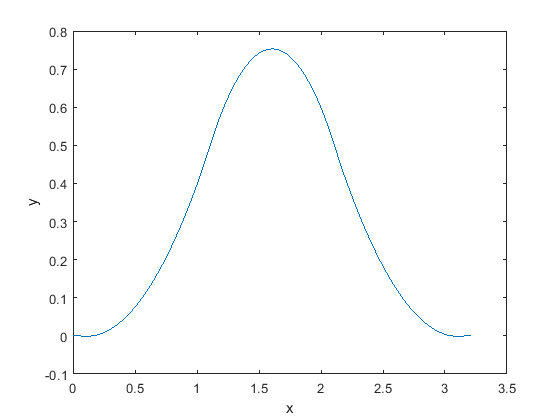
\includegraphics[width=5cm,keepaspectratio]{./graphics/blf}
    \caption{Graphic output of Example~\ref{sec_ex_mss}.}
\end{figure}

%%%%%%%%%%%%%%%%%%%
% EOF
%%%%%%%%%%%%%%%%%%%

% !TeX encoding = UTF-8 Unicode
% !TeX root = manual.tex
% !TeX spellcheck = en_GB

\chapter{Code to produce the images and results from~\cite{Mej20}}

All figures are printed with Matlab. In order to reproduce them, additionally the 
\verb|export_fig| package, available at \href{https://de.mathworks.com/matlabcentral/fileexchange/23629-export_fig}%
{\emph{mathworks.com/matlabcentral/fileexchange/23629}} 
is necessary.
Furthermore, the following anonymous functions are used.

{\small%
\begin{lstlisting}
clc;
warning('off','MATLAB:MKDIR:DirectoryExists');
warning('off','MATLAB:LargeImage');

DPI='-r600';        %resolution
EXT='-pdf';         %default file format
BASE='.';           %base folder
AA='-a1';           %anti-aliasing. a1=off, a3=a lot
LGREY=[.6 .6 .6];   %color for light-grey
DGREY=[.4 .4 .4];
BLACK=[0 0 0];      %color for black
DOTSIZE=4;          %size of markers and dots
LINESIZE=.5;        %width of lines
FONTSIZE=8;         %font size

% %%%%%%%%%%%%%%%%%%%%%%%%
set(groot,'defaultAxesTickLabelInterpreter','latex');  
set(groot,'defaulttextinterpreter','latex');
set(groot,'defaultLegendInterpreter','latex');

FIGURE = @() figure('Units','Centimeters','Position',[0 0 25 25]);
TITLE = @(T) title(T,'Interpreter','latex');
AXISE = @(A) eval('axis(''equal''); axis(A)');
AXIS = @(A) eval('axis(A)');
LABEL = @(X,Y) eval(['xlabel(X,''Interpreter'',''Latex'');'...
   'ylabel(Y,''Interpreter'',''Latex'');']);
TICKS = @(X,Y) eval('xticks(X); yticks(Y);');
TICKLABELS = @(X,Y) eval('xticklabels(X); yticklabels(Y);');
SIZE = @(X,Y) set(gca,'Units','Centimeters','Position',[3 3 3*X 3*Y]);
SIZE1 = @() set(gca,'Units','Centimeters','Position',[3 3 15 1]);
TEXT = @(X,Y,T) text(X, Y, T,'Interpreter','Latex','Fontsize',FONTSIZE);
POST = @() eval(['set(findall(gcf,''-property'',''FontSize''),''FontSize'',' ...
   num2str(FONTSIZE) ' );'...
   'set(gca,''TickLabelInterpreter'', ''Latex'');'...
   'set(gcf, ''Color'', ''w'');'...
   'set(gca,''XMinorTick'',''off'',''YMinorTick'',''off'');'...
   'box on']);    
SAVE = @(FOLDER,NAME,EXT) eval(['mkdir(fullfile('''',''' BASE ''', FOLDER));'...
   'export_fig(fullfile('''', ''' BASE ''',FOLDER,NAME), ''-grey'', ''' DPI ...
   ''', ''' AA ''', ''' EXT ''', ''-dCompatibilityLevel=1.4'');'...
'fprintf(''%s/%s finished\n=============================================\n' ...
'=============================================\n'',FOLDER,NAME);']);
% %%%%%%%%%%%%%%%%%%%%%%%%
\end{lstlisting}%
}

\newpage
\section{Figure 1}
\begin{center}
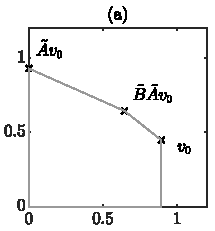
\includegraphics{./graphics/invpoly_1}
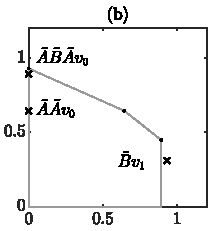
\includegraphics{./graphics/invpoly_2}
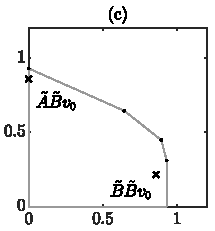
\includegraphics{./graphics/invpoly_3}
\end{center}

{\small%
\begin{lstlisting}
FIGURE(); hold on;
AE=[0 1.2 0 1.2]; TE=[0 .5 1]; %Axis and Ticks
A=[0 0;1 1]; B=[1 1;0 1]; cA={A,B}; 
tjsr(cA,'plot','polytope','fastnorm',0,'ordering',{[2 1 1]'});
Pi=B*B*A; rhoc=rho(Pi)^(1/3); At=A/rhoc; Bt=B/rhoc; Pit=Pi/rhoc^3; v1=1/sqrt(5)*[2;1];
V=[v1 At*v1 Bt*At*v1];
plotm(V,'x','Color',BLACK,'MarkerSize',DOTSIZE);
plotm(([V [0;0] [max(V(1,:));0] [0;max(V(2,:))]]),'hull','-','Color',LGREY,'LineWidth',LINESIZE);
TEXT(1,.4,'$v_0$');
TEXT(0.05,1.05,'$\tilde{A}v_0$'); 
TEXT(.7,.75,'$\tilde{B}\tilde{A}v_0$'); %cyclic root
SIZE(1,1); AXISE(AE); TICKS(TE,TE); LABEL('',''); TITLE('(a)'); POST();
SAVE('.','invpoly_1',EXT);
FIGURE(); hold on;
%V=V;
Vnew=[Bt*v1 At*At*v1 At*Bt*At*v1];
plotm(([V [0;0] [max(V(1,:));0] [0;max(V(2,:))]]),'hull','-','Color',LGREY,'LineWidth',LINESIZE);
plotm(V,'.','Color',BLACK,'MarkerSize',DOTSIZE);
plotm(Vnew,'x','Color',BLACK,'MarkerSize',DOTSIZE);
TEXT(.6,.3,'$\tilde{B}v_1$'); TEXT(.05,.65,'$\tilde{A}\tilde{A}v_0$'); TEXT(.05,1,'$\tilde{A}\tilde{B}\tilde{A}v_0$'); %new vertices
SIZE(1,1); AXISE(AE); TICKS(TE,TE); LABEL('',''); TITLE('(b)'); POST();
SAVE('.','invpoly_2',EXT);
FIGURE(); hold on;
V=[V Bt*v1]; 
Vnew=[Bt*Bt*v1 At*Bt*v1];
plotm(([V [0;0] [max(V(1,:));0] [0;max(V(2,:))]]),'hull','-','Color',LGREY,'LineWidth',LINESIZE);
plotm(V ,'.','Color',BLACK,'MarkerSize',DOTSIZE);
plotm(Vnew,'x','Color',BLACK,'MarkerSize',DOTSIZE);
TEXT(.55,.1,'$\tilde{B}\tilde{B}v_0$'); TEXT(.05,.7,'$\tilde{A}\tilde{B}v_0$'); %new vertices
SIZE(1,1); AXISE(AE); TICKS(TE,TE); LABEL('',''); TITLE('(c)'); POST();
SAVE('.','invpoly_3',EXT);
\end{lstlisting}%
}

\newpage
\section{Example 4.3}
\begin{center}
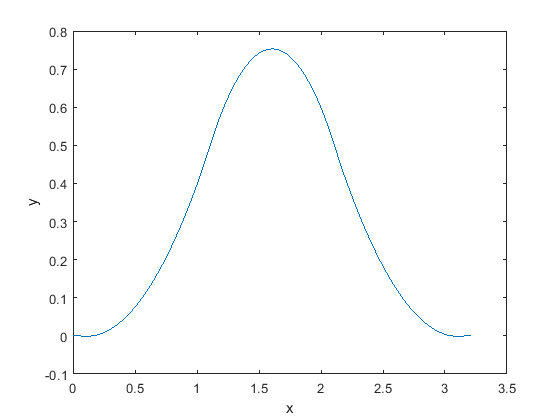
\includegraphics{./graphics/blf}	
\end{center}
\begin{lstlisting}
S = getS( 'a',sym(1/12)*[3 3 4 3 3 4 3 3 4 3 3].', 'M',-3, 'D',[-2 -1 0] )
[T,Om] = transitionmatrix( S )
V = constructVt( Om, 0 )
TV = restrictmatrix( T, V )
vdisp( -12.*TV )

tjsr( TV ); %with balancing
tjsr( TV, 'nobalancing' );

%%%%%%%%%%

FIGURE();
S=getS({1/12*[3 3 4 3 3 4 3 3 4 3 3]',-3,[]});
blf(S,'plot',{'Color',DGREY,'LineWidth',1}); 
SIZE(1.5,1); AXIS([-4 2 0 .3]); TICKS([-4 -2 0 2 4],[0 0.1 0.2 0.3]); LABEL('',''); POST();
SAVE('.','blf',EXT);
\end{lstlisting}


\section{Example 4.4}
{\small%
\begin{lstlisting}
E1 = [2 1;-1 2];
E2 = [2 0; 2 1];
tjsr( {E1,E2}, 'ordering',{[1 2]' [2 0]'}, 'smpflag',[0 1], ...
   'balancingvector',[1 0.95], 'invariantsubspace','none' )
\end{lstlisting}%
}

\section{Table 1 / Table 2}
The results are obtained with scripts similar to
{\small%
\begin{lstlisting}
dim = 10;
T = [];
i = 0;
while( i<10);
    M = tgallery( 'rand_gauss', dim, 2, 'norm' );
    [r,info] = tjsr( M );
    if( numel(r)==1 && info.info.errorcode<0 );
        i = i+1; 
        T(end+1) = info.counter.treetime; end;  end;
mean(T)
\end{lstlisting}%
}


\section{Table 3}
The results are obtained with scripts similar to
{\small%
\begin{lstlisting}
dim = 2;
J = 4;
i = 0;
[GRIP,MODGRIP] = deal( [] );
while( i<3 );
    M = tgallery( 'rand_gauss', dim, J, 'rho' );
    [r,info] = tjsr( M );
    if( numel(r)~=1 || info.info.errorcode>=0 );
        fprintf( ' Modified Invariant polytope algorithm did not find s.m.p..\n' );
        continue; end;
    i=i+1;
    
    [~,~,val] = findsmpold( M, 'gripenberg' );
    if( abs(val.jsrbound(1)-r)<1e-12 )
        GRIP(end+1) = val.time;
    else
        GRIP(end+1) = inf; end;
    
    [~,~,val] = findsmpold( M );
    if( abs(val.jsrbound(1)-r)<1e-12 )
        MODGRIP(end+1) = val.time;
    else
        MODGRIP(end+1) = false; end; end;
\end{lstlisting}%
}

\section{Example 5.1 / Table 4 / Table 5}
The results are obtained with scripts similar to
{\small%
\begin{lstlisting}
X = tgallery('mejstrik_119');
cmodgrip = findsmpold( X, 'maxsmpdepth',120 )
cgrip = findsmpold( X, 'gripenberg', 'delta',1, 'maxsmpdepth',120, 'v',2 )
cgen = findsmpold( X, 'genetic' )

C15 = tgallery('mejstrik_Cn',15)
cmodgrip = findsmpold( C15, 'maxsmpdepth',20 )
\end{lstlisting}%
}

\section{Table 6 / Table 7}
The results are obtained with scripts similar to
{\small%
\begin{lstlisting}
D = {[1 1],[1 -1],[-1 1],[-1 -1]};
C = codecapacity( D );
tjsr( C, 'v',2, 'maxsmpdepth',2 )
\end{lstlisting}%
}

\section{Table 8 / Figure 5}
\begin{center}
    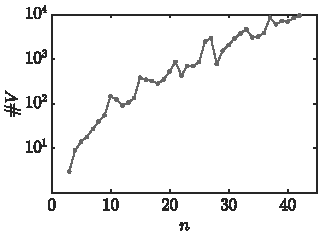
\includegraphics{./graphics/nVdaub}$\qquad$
    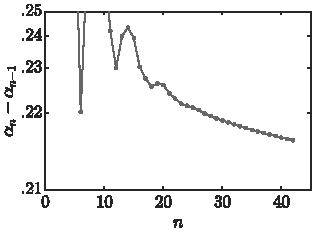
\includegraphics{./graphics/aldaub}
\end{center}
The figure is printed using
{\small%
\begin{lstlisting}
FIGURE(); 
V=[0 3 9 14 18 27 40 55 147 123 91 105 134 386 346 324 282 346 529 868 433 707 701 861 2471 2952 777 1545 2078 2898 3791 4692 3047 3191 3887 8529 6035 7142 6909 8343 9508];
n=[2 3 4 5 6 7 8 9 10 11 12 13 14 15 16 17 18 19 20 21 22 23 24 25 26 27 28 29 30 31 32 33 34 35 36 37 38 39 40 41 42];
semilogy(n,V,'o-','Color',DGREY,'MarkerSize',1,'MarkerFaceColor',DGREY);
set(findall(gcf,'-property','YMinorTick'),'YMinorTick','off')
SIZE(1.5,1); AXIS([0 45 1 10^4]); TICKS([0 10 20 30 40],[1e1 1e2 1e3 1e4]); LABEL('$n$','$\#V$'); TITLE(''); POST();
SAVE('.','nVdaub',EXT);

FIGURE();
n=[2 3 4 5 6 7 8 9 10 11 12 13 14 15 16 17 18 19 20 21 22 23 24 25 26 27 28 29 30 31 32 33 34 35 36 37 38 39 40 41 42];
al=[0.55001 1.08783 1.61793 1.96896 2.18914 2.46041 2.76082 3.07361 3.36139 3.60347 3.83348 4.07348 4.31676 4.55612 4.78644 5.01380 5.23917 5.46532 5.69108 5.91500 6.13779 6.35958 6.58096 6.80198 7.02250 7.24241 7.46187 7.68091 7.89962 8.11801 8.33605 8.55379 8.77123 8.98841 9.20533 9.42202 9.63847 9.85474 10.07073 10.28656 10.50220];
diffal=diff([0 al]);
semilogy(n,diffal-.2,'o-','Color',DGREY,'MarkerSize',1,'MarkerFaceColor',DGREY)
SIZE(1.5,1); AXIS([0 45 .01 .05]); TICKS([0 10 20 30 40],[0.01 .02 .03 .04 .05]); LABEL('$n$','$\alpha_n-\alpha_{n-1}$'); TICKLABELS({'0', '10', '20', '30', '40'},{'.21','.22','.23','.24','.25'});
SAVE('.','aldaub',EXT);
\end{lstlisting}%
}

The results from the table are obtained with scripts similar to
{\small%
\begin{lstlisting}
A = daubechiesmatrix( 10 );
tjsr( A, 'v',2 )
\end{lstlisting}%
}


\end{document}


















%%%%%%%%%%%%%%%%%
% EOF
%%%%%%%%%%%%%%%%%